
\chapter{MOTION PRIMITIVE TRANSITION:WALK AND STANCE}
\label{chap:stance}
\ifpdf
    \graphicspath{{WalkStance/WalkstanceFigs/PNG/}{WalkStance/WalkStanceFigs/PDF/}{WalkStance/WalkStanceFigs/}}
\else
    \graphicspath{{WalkStance/WalkStanceFigs/EPS/}{WalkStance/WalkStanceFigs/}}
\fi



\section{Motion Primitives}
For Bipedal Walking, when the heel strike happens, it the passive walker don't get enough velocity, it will stop walk and rest at the heel strike pos.
This is posture is stable, then we got another motion primitive: the stance, as show in figure ~\ref{fig:bipedalstance}



\begin{figure}[!htbp]
  \begin{center}
    \leavevmode
    \ifpdf
      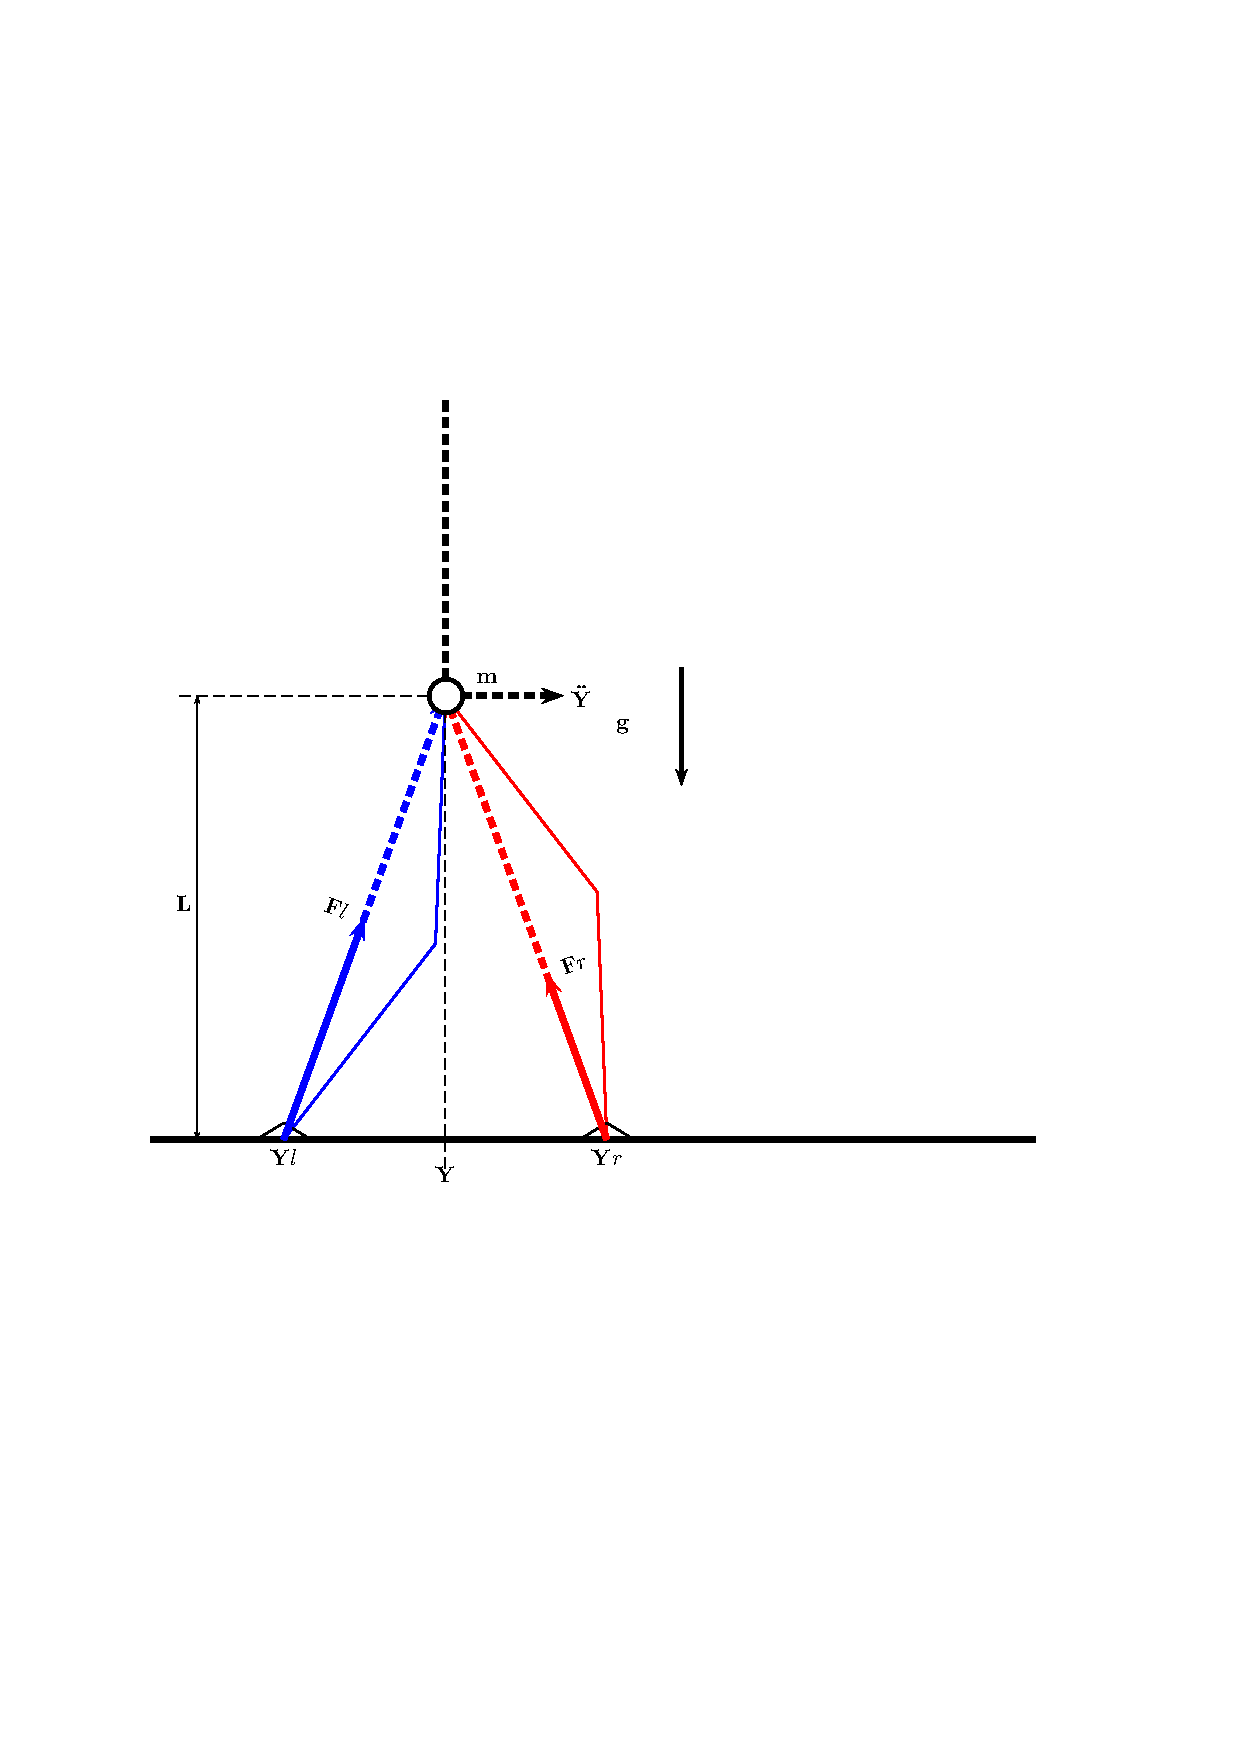
\includegraphics[height=6in]{stancefigure}
    \else
      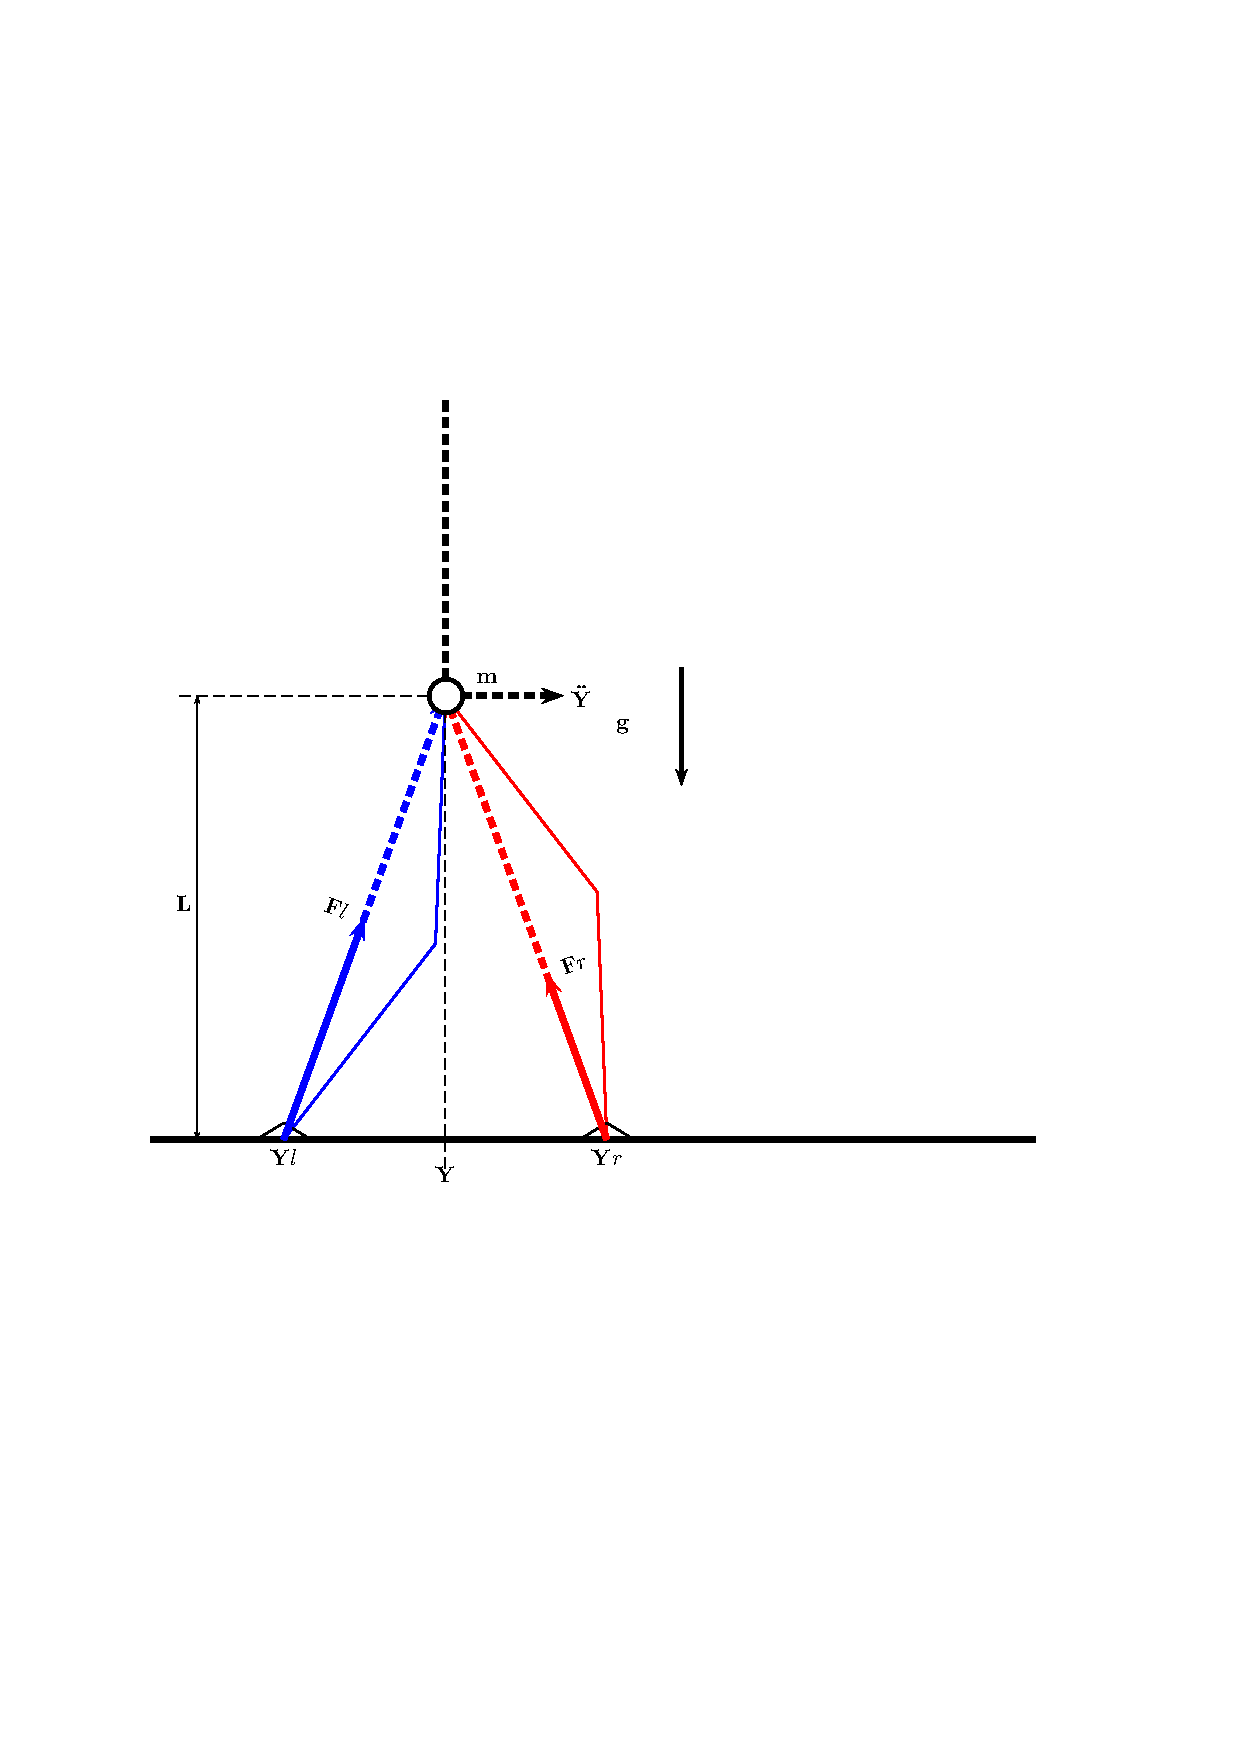
\includegraphics[width=0.7\textwidth]{stancefigure}
    \fi
    \caption{The Stance Motion Primitives}
    \label{fig:bipedalstance}
\end{center}
\end{figure}



usually when people stands, the two legs are almost straight, and the heigt is almost constant.
It is not necessary to consider the full details of four link leg model.
we can simplify the stance mode as a point supported by two straight legs. 
For normal human stance, high change will be less than 5\%, we suppose it is constant.
we only consider the horizontal displacement.
this simplified model is proposed by although is simple, but capture the key characters of stancing~\citep{stephens2009modeling}.
use this method, we show the stance motion in the following figures ~\ref{fig:stanceopostures}

\begin{figure}[!htbp]
  \begin{center}
    \leavevmode
    \ifpdf
      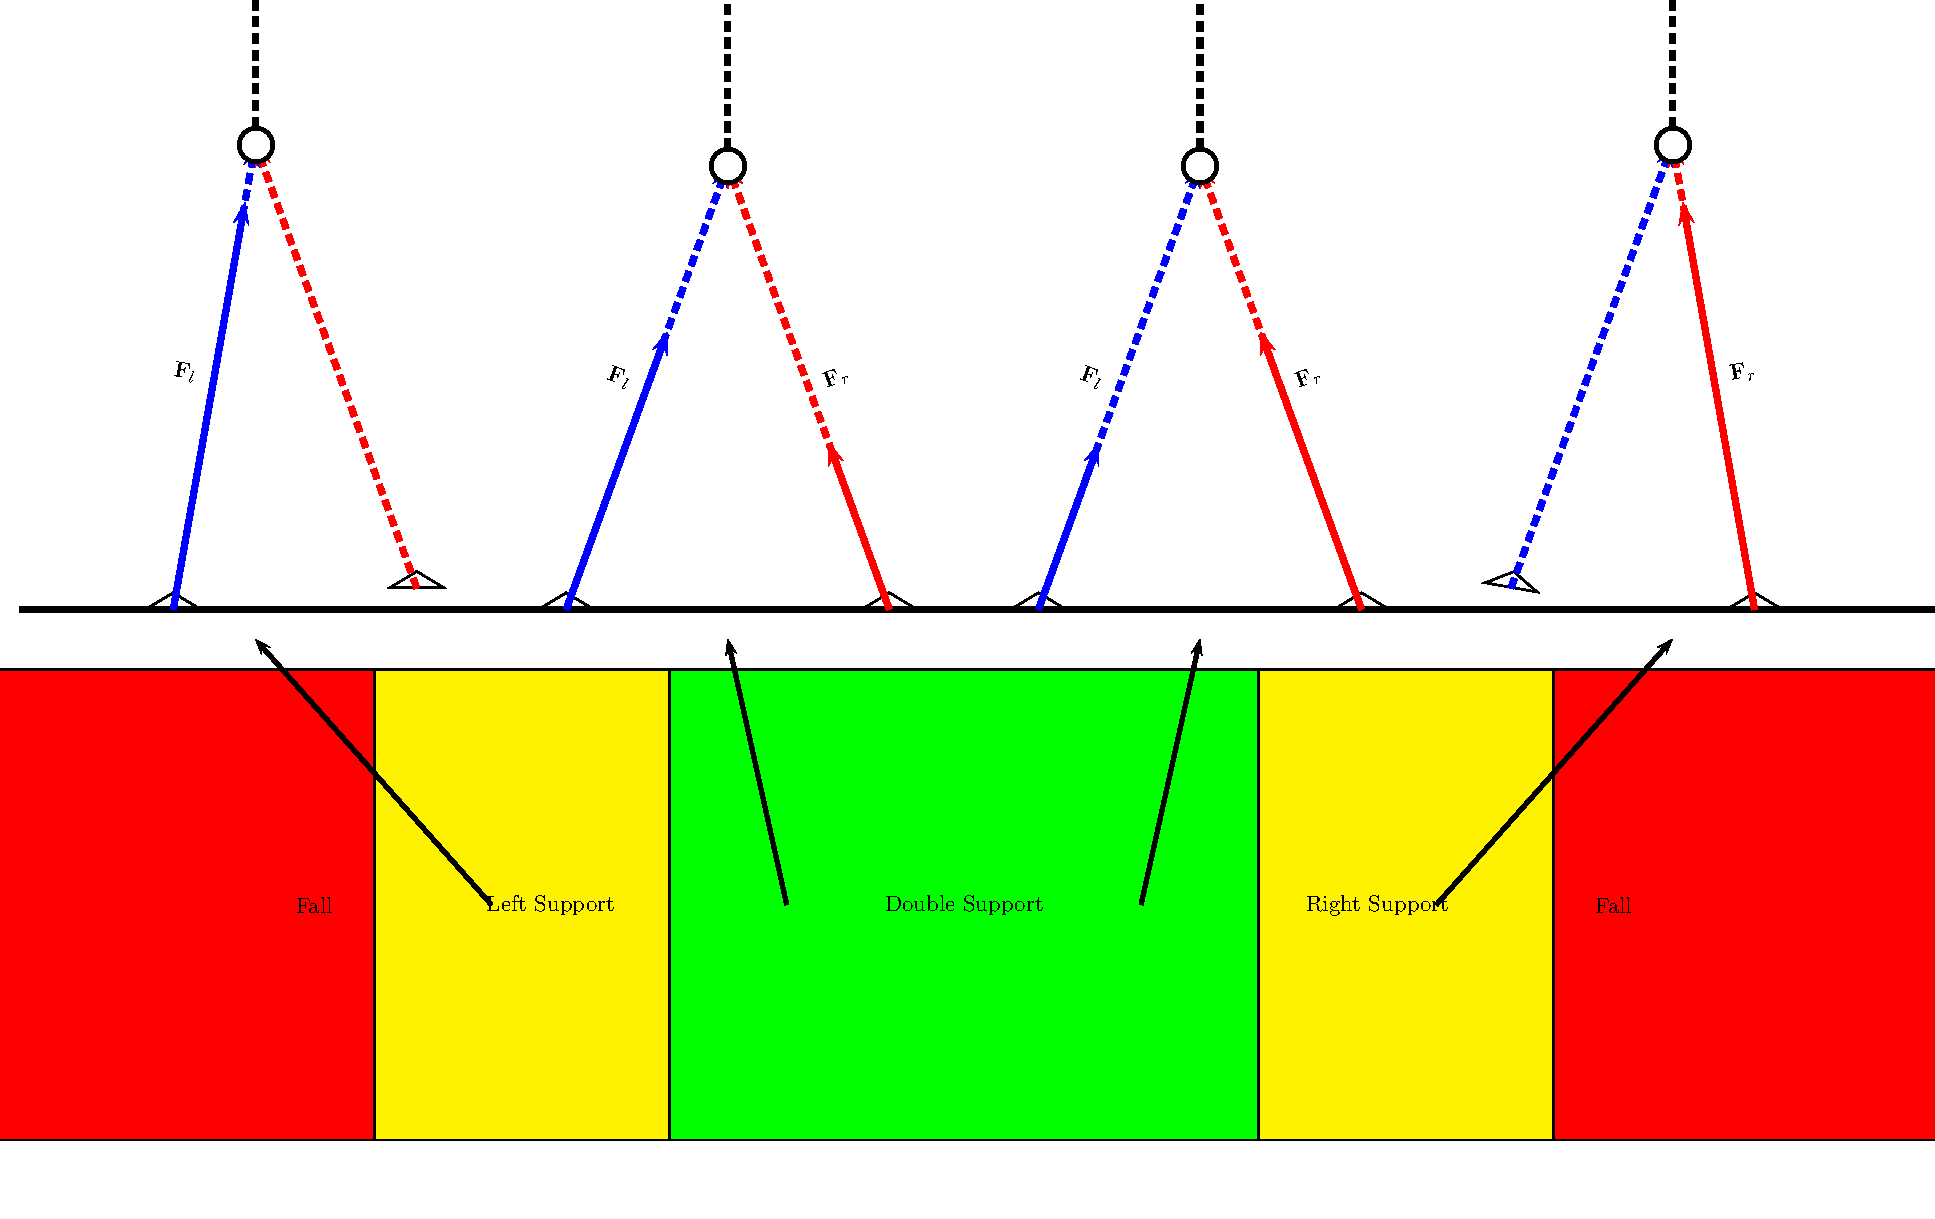
\includegraphics[height=6in]{stanceConfigure}
    \else
      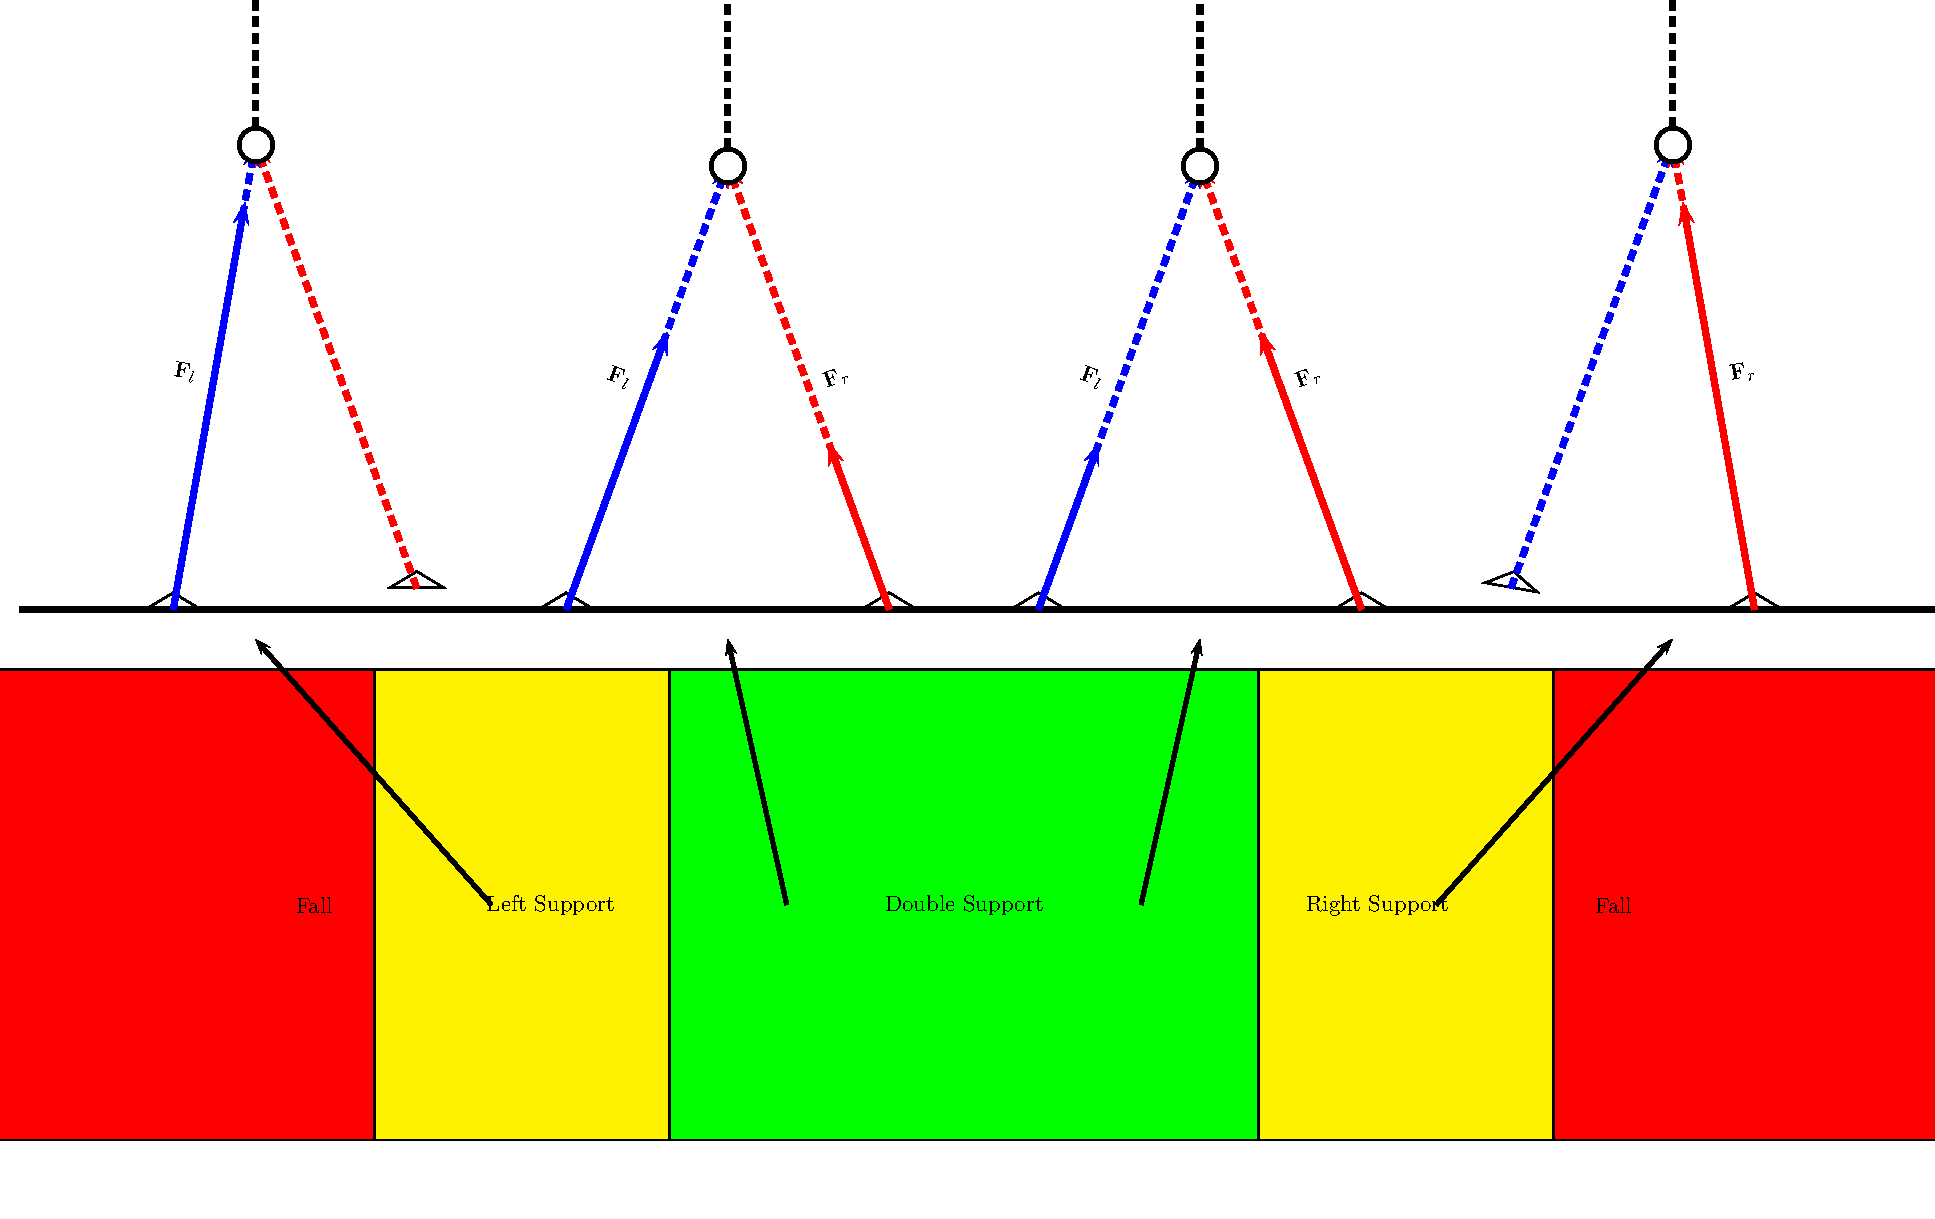
\includegraphics[width=0.7\textwidth]{stanceConfigure}
    \fi
    \caption{The Stance Motion Posture}
    \label{fig:stancepostures}
\end{center}
\end{figure}

the stance is easy for human, but the dynamic is not trifle.
stance is not continues system, the dynamic involves three phase

\begin{itemize}
\HiItem{Double Support}
When the horitontal displace model is small, people stand with two legs support.
the motion is governed by the gravity.
\[
\ddot{q}=\frac{g}{L}w_r(y_m-y_r)+\frac{g}{L}w_l(y_m-y_l)
\]


but usually some intuitive strategy is applied.
if the two legs generate torque to maintain the posture, the two torques should not be equal,
if the centre moving to the left, then the left torque will generate more torque.
if the centre moving to the right, then the right leg will generate more torque.
suppose the relationship is linear.
then we get the following intuitive control stance equation, which we used as the mechanical oscillator.
\begin{equation}
\label{eq:stanceequation}
\ddot{q}=\frac{g}{L}w_r(y_m-y_r)+\frac{g}{L}w_l(y_m-y_l)+\frac{\tau_L+\tau_R}{mL}
\end{equation}



\HiItem{Single Leg Support}
if the there is a big horizontal displacement, there people will stand with single leg.
passively, the equation is 
\[
\ddot{q}=\frac{g}{L}q
\]
and intuitive even controlled
\begin{equation}
\label{equ:singlestand}
\ddot{q}=\frac{g}{L}q+\frac{y_{L,R}}{L}\tau_{L,R}
\end{equation}

\HiItem{Fall and Walk}
if the displacement is even bigger,then the walker will move out the support region.
for a human, where the stance region is depends on the  height and the step size.
And the goal of balancing is to maintain the system state within the support region.

Usually, it will result two motion sequences, whether it will start to walk for it will fall


\end{itemize}

\section {Stance Control}
\subsection{Entraintment}

without damping effects, the original system is similar to mass spring system.
It wil vibrate continentally.

the phase plot is shown in
\begin{figure}[!htbp]
  \begin{center}
    \leavevmode
    \ifpdf
      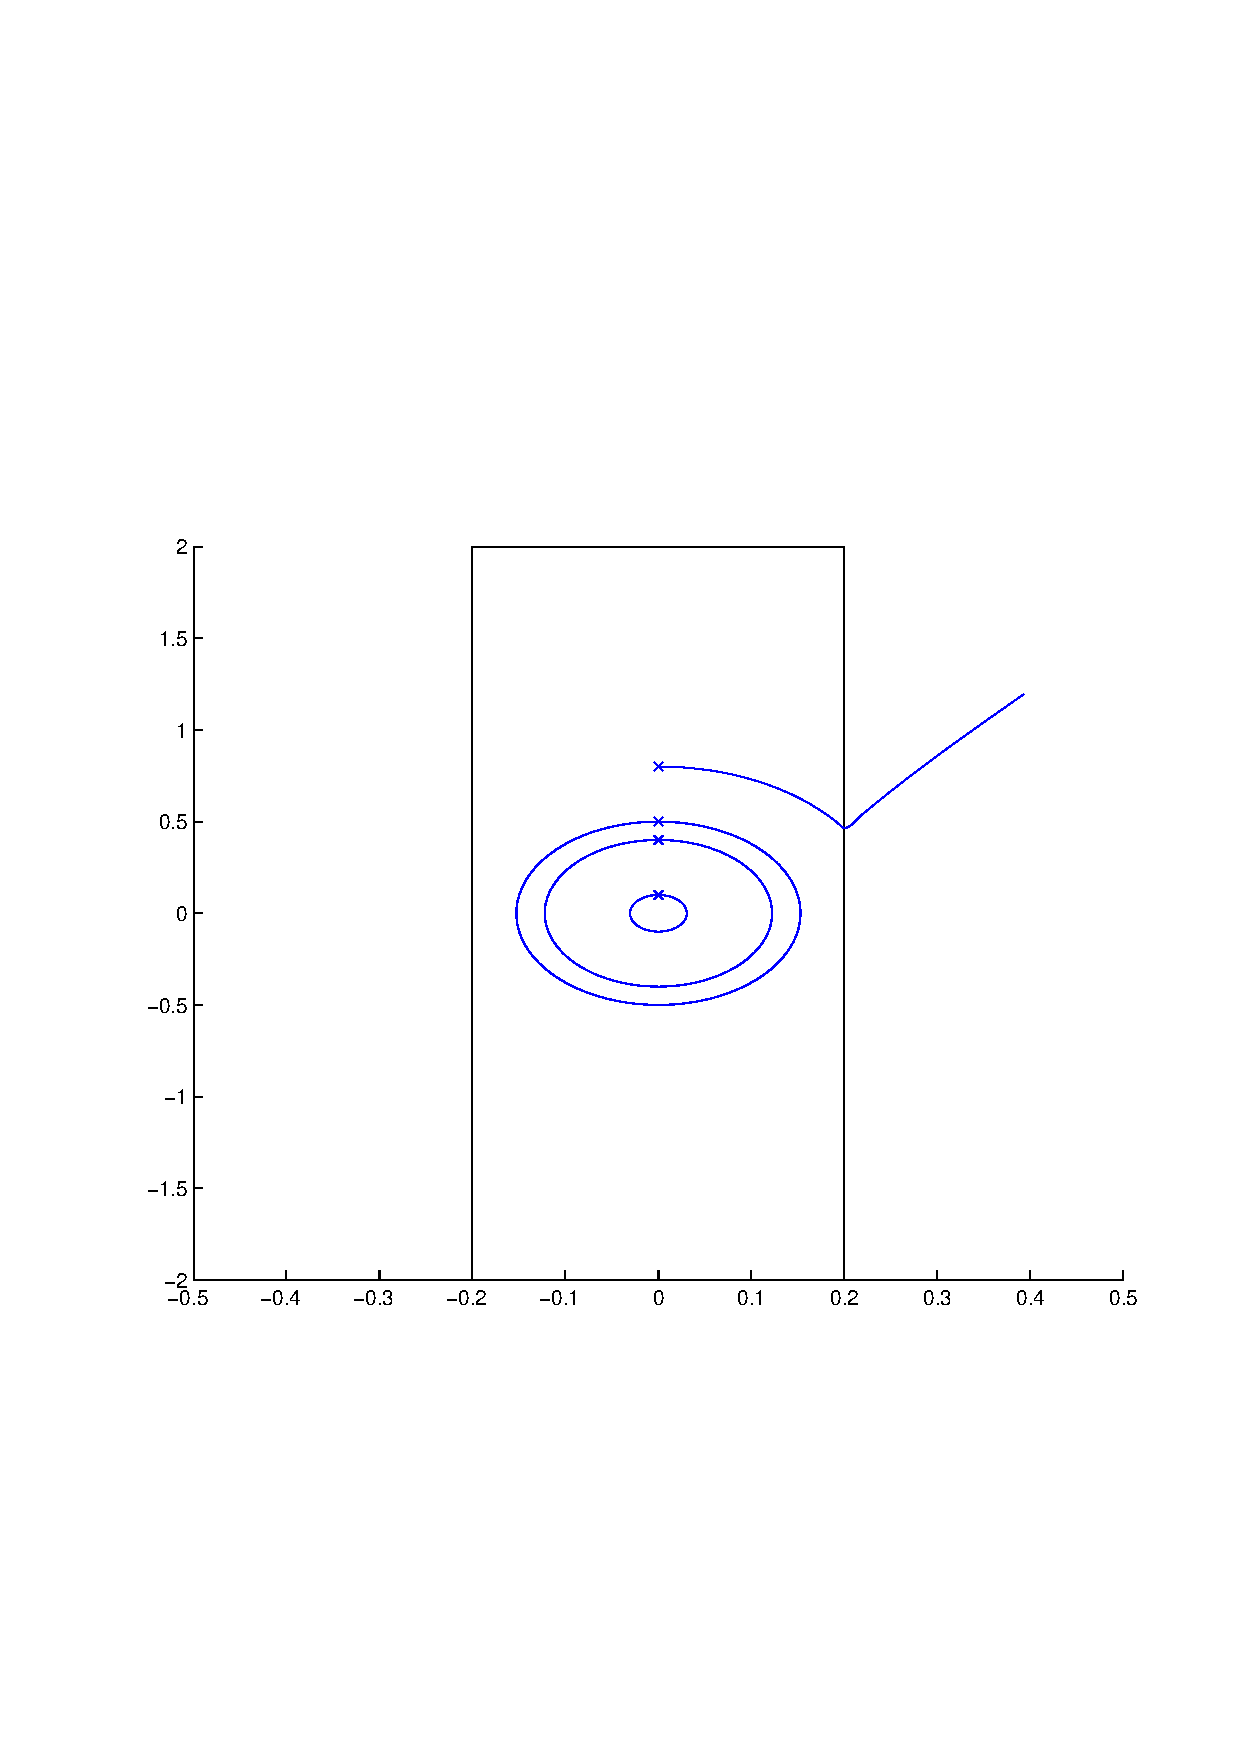
\includegraphics[height=6in]{uncontrolled}
    \else
      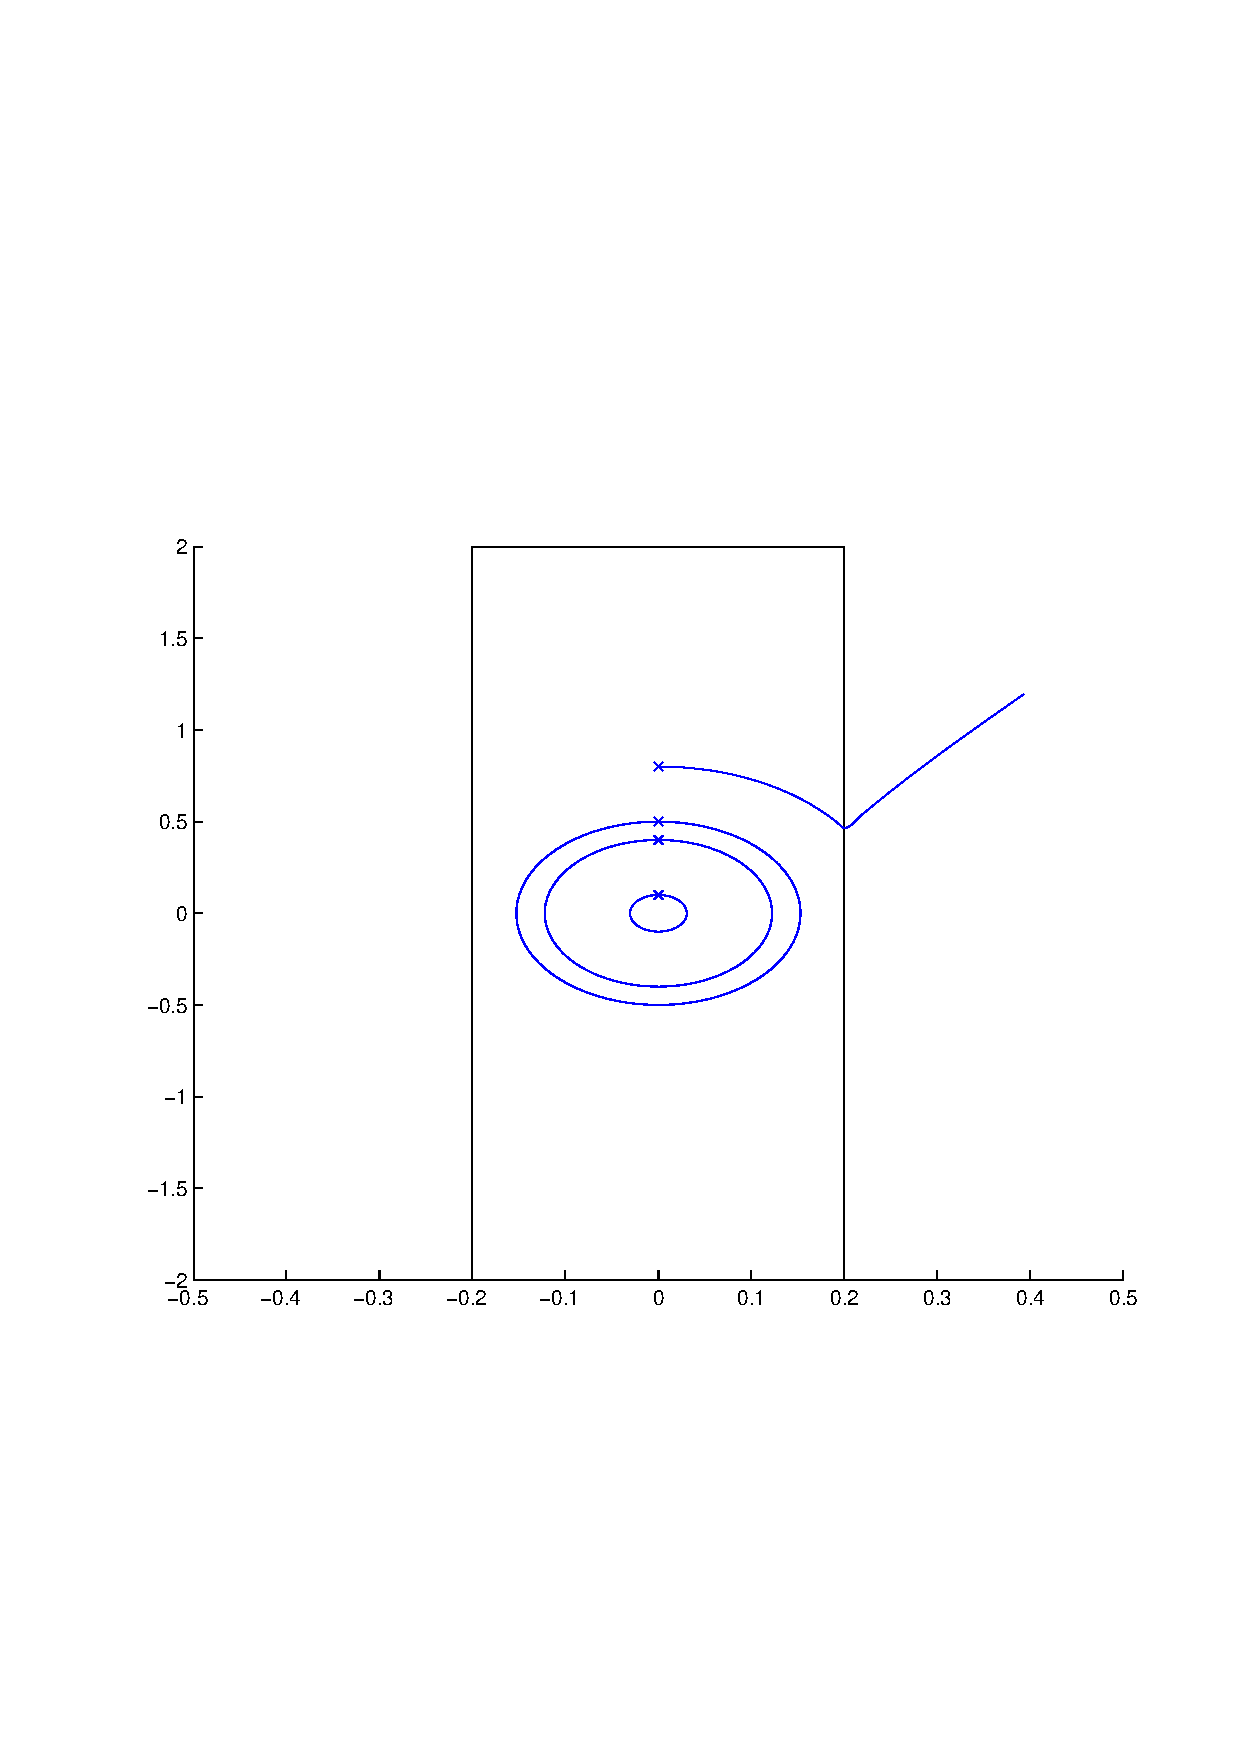
\includegraphics[width=0.7\textwidth]{uncontrolled}
    \fi
    \caption{un controlled motion}
    \label{fig:stancepostures}
\end{center}
\end{figure}

if the initial speed is higher, then it will move out the support region.



while in our method ,by coupling neural system the oscillator, it will form a limit circle,
but for this situation of standing, limit circle doesn't not boost the stability,because the boundary is fixed,
neural oscillator will not modify the boudary,and it is impossible for mechanical system to converge to the limit circle within 1/4 period.
thus we make the output of the output of neural controller very small $\uout$.

Limit Circle is useful for it can make stance start to vibrate at a constant speed, this will be very helpful when we start from stance to walk.

\subsection{Local Invariant Control}
All the three group controller can be used,but basically only two control method are useful.
\subsubsection*{Time Scaling}
The first is time scaling $\gts$
as show in figure
\begin{figure}[!htbp]
  \begin{center}
    \leavevmode
    \ifpdf
      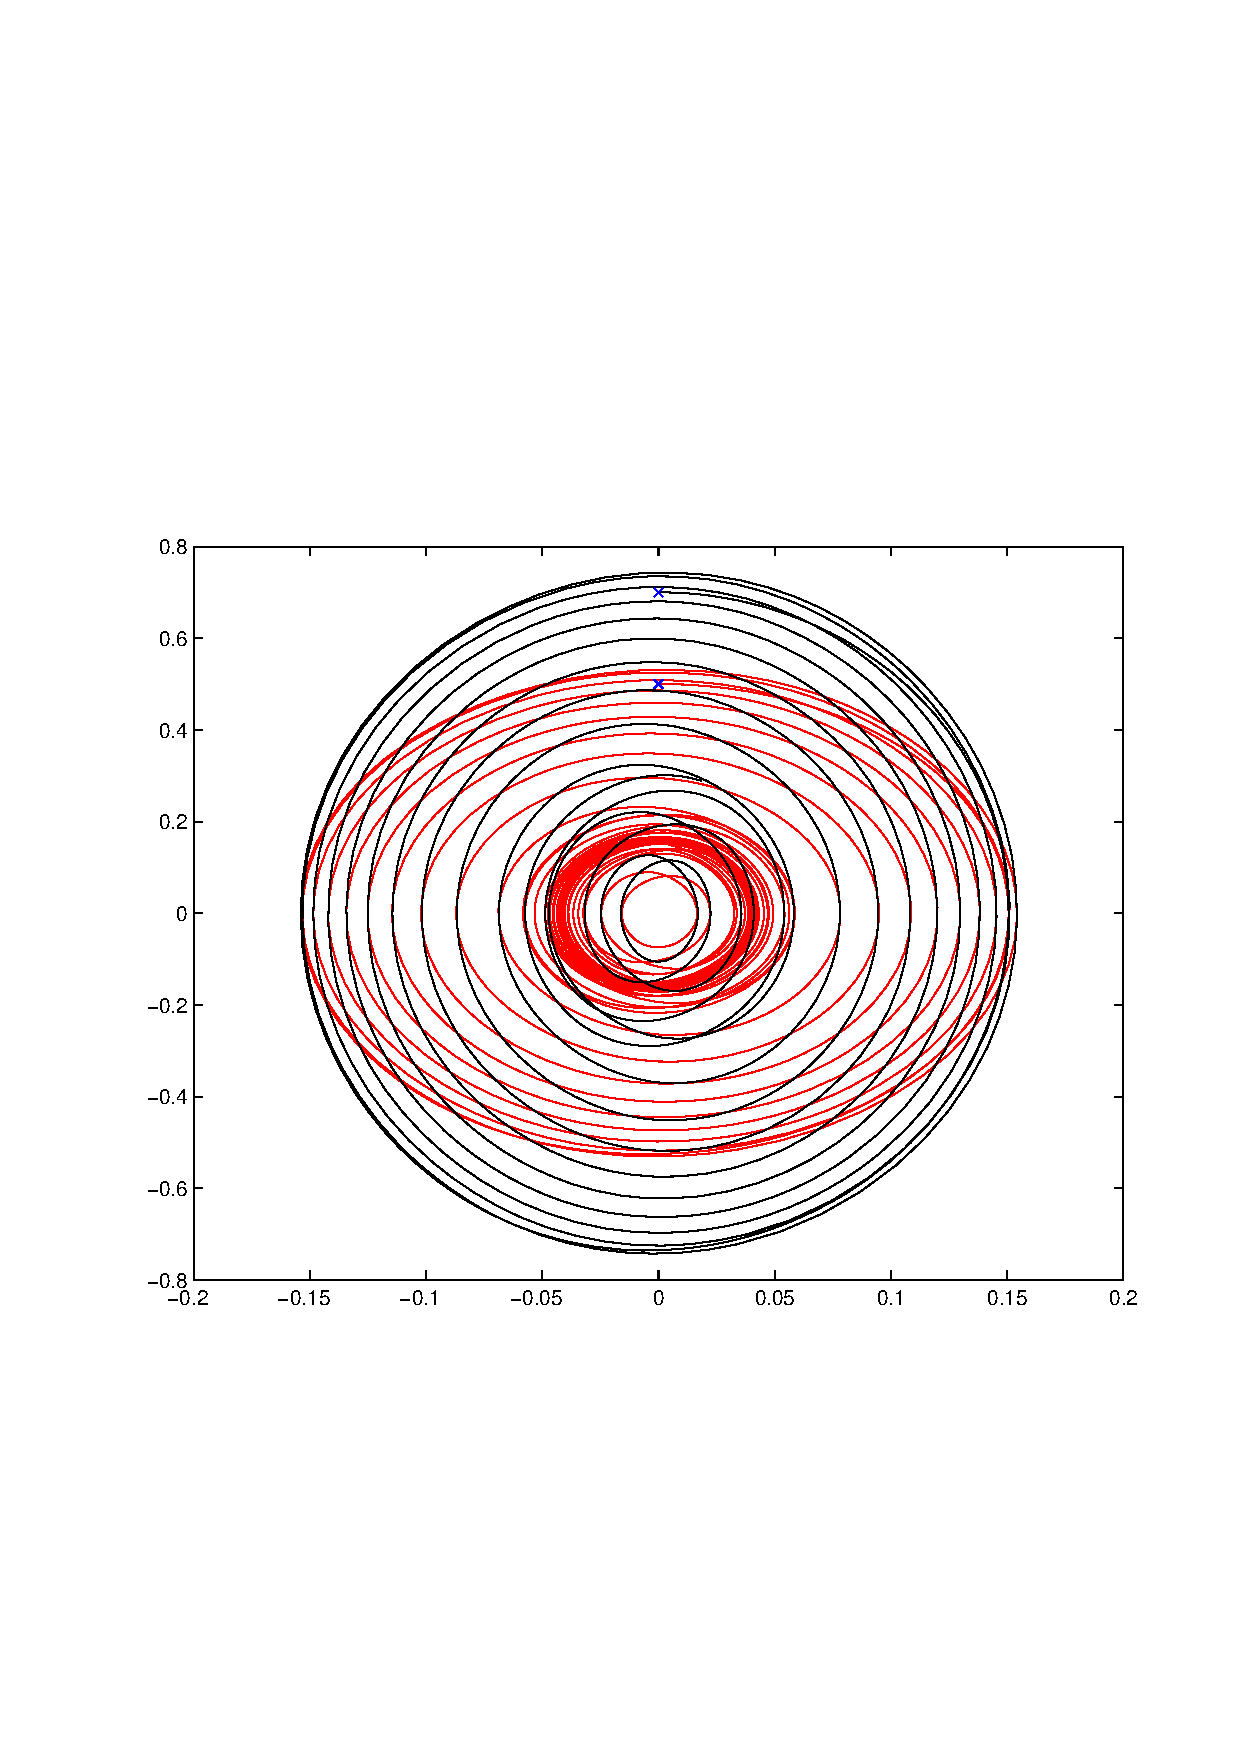
\includegraphics[height=6in]{TimeScaling}
    \else
      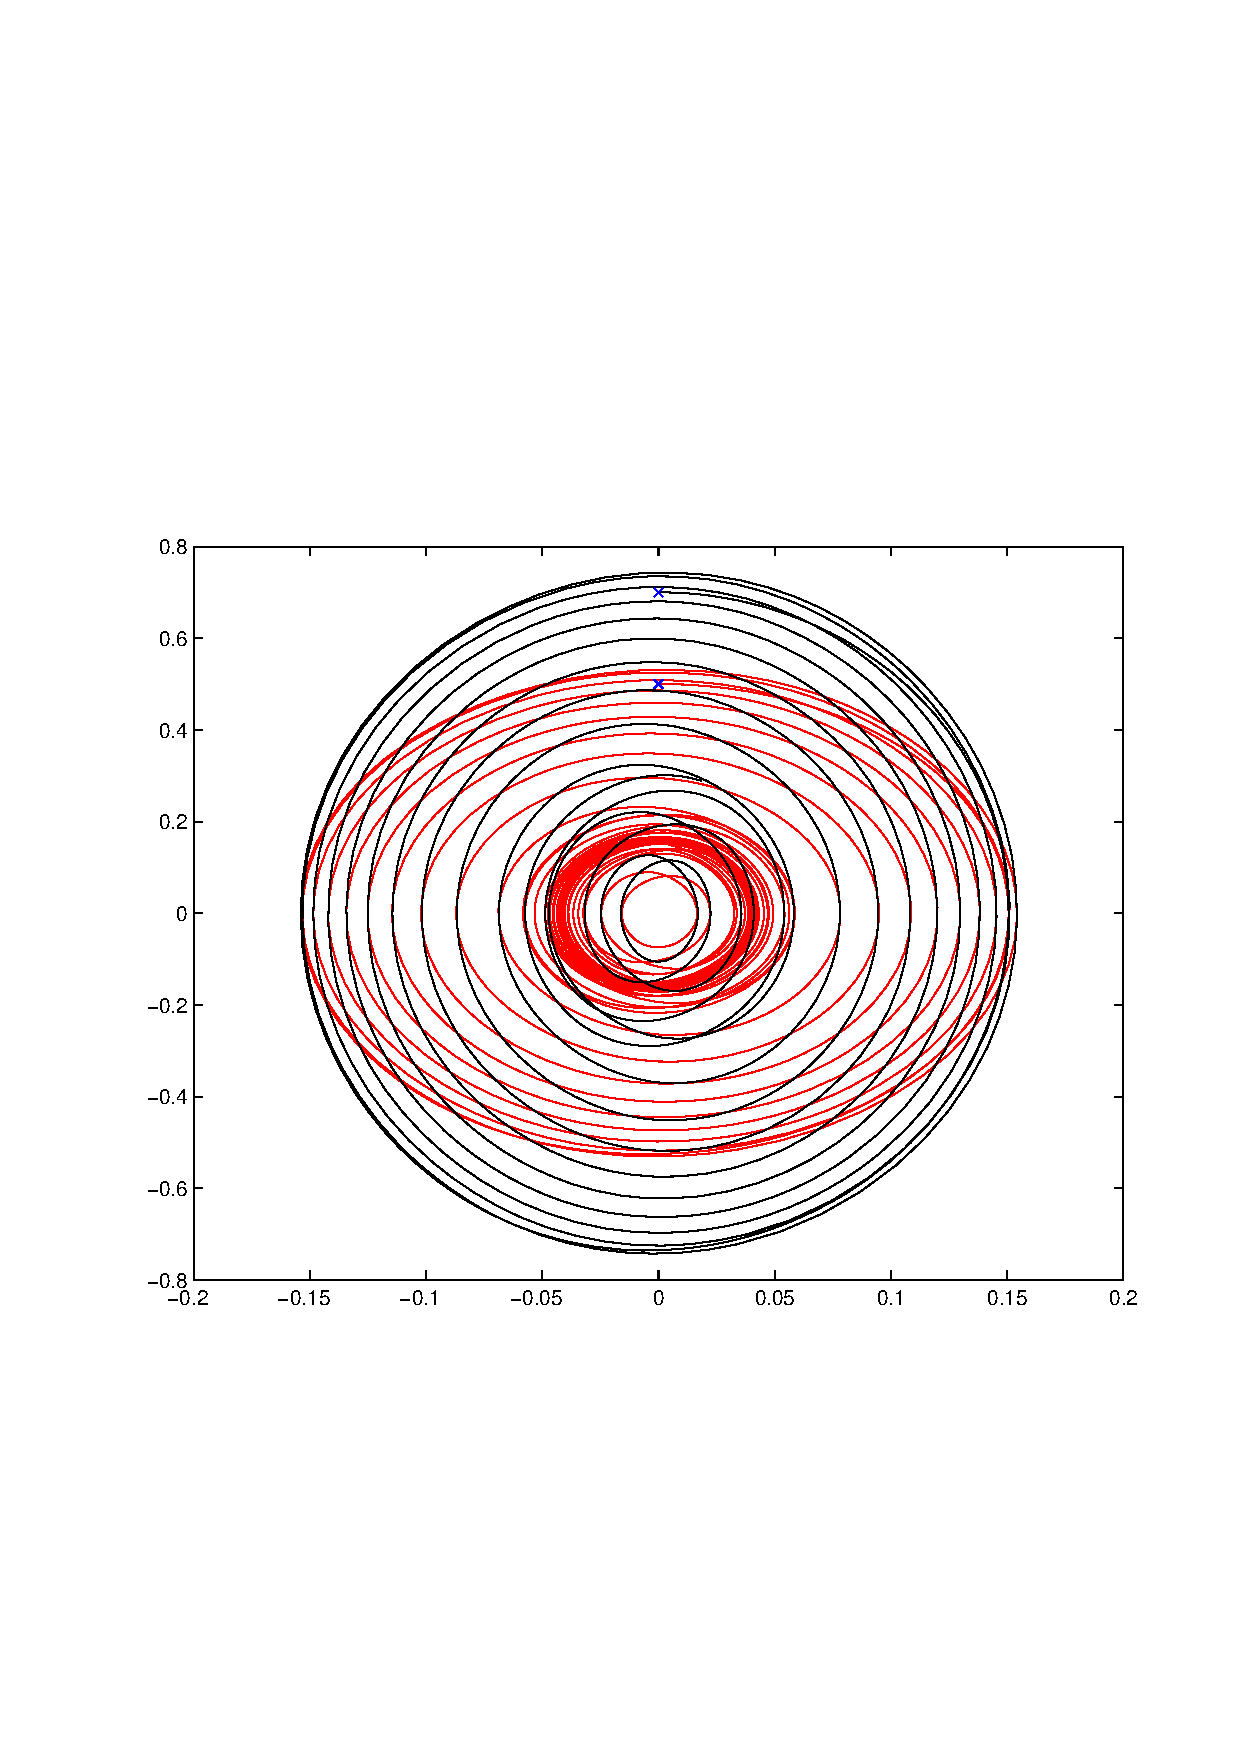
\includegraphics[width=0.7\textwidth]{TimeScaling}
    \fi
    \caption{Time Scaling}
    \label{fig:stanceTimeScaling}
\end{center}
\end{figure}
The Time Scaling will enlarge the basin of attraction to include high speed state.

The falling motion is show in the figure ~\ref{fig:stancefall}
\begin{figure}[!htbp]
  \begin{center}
    \leavevmode
    \ifpdf
      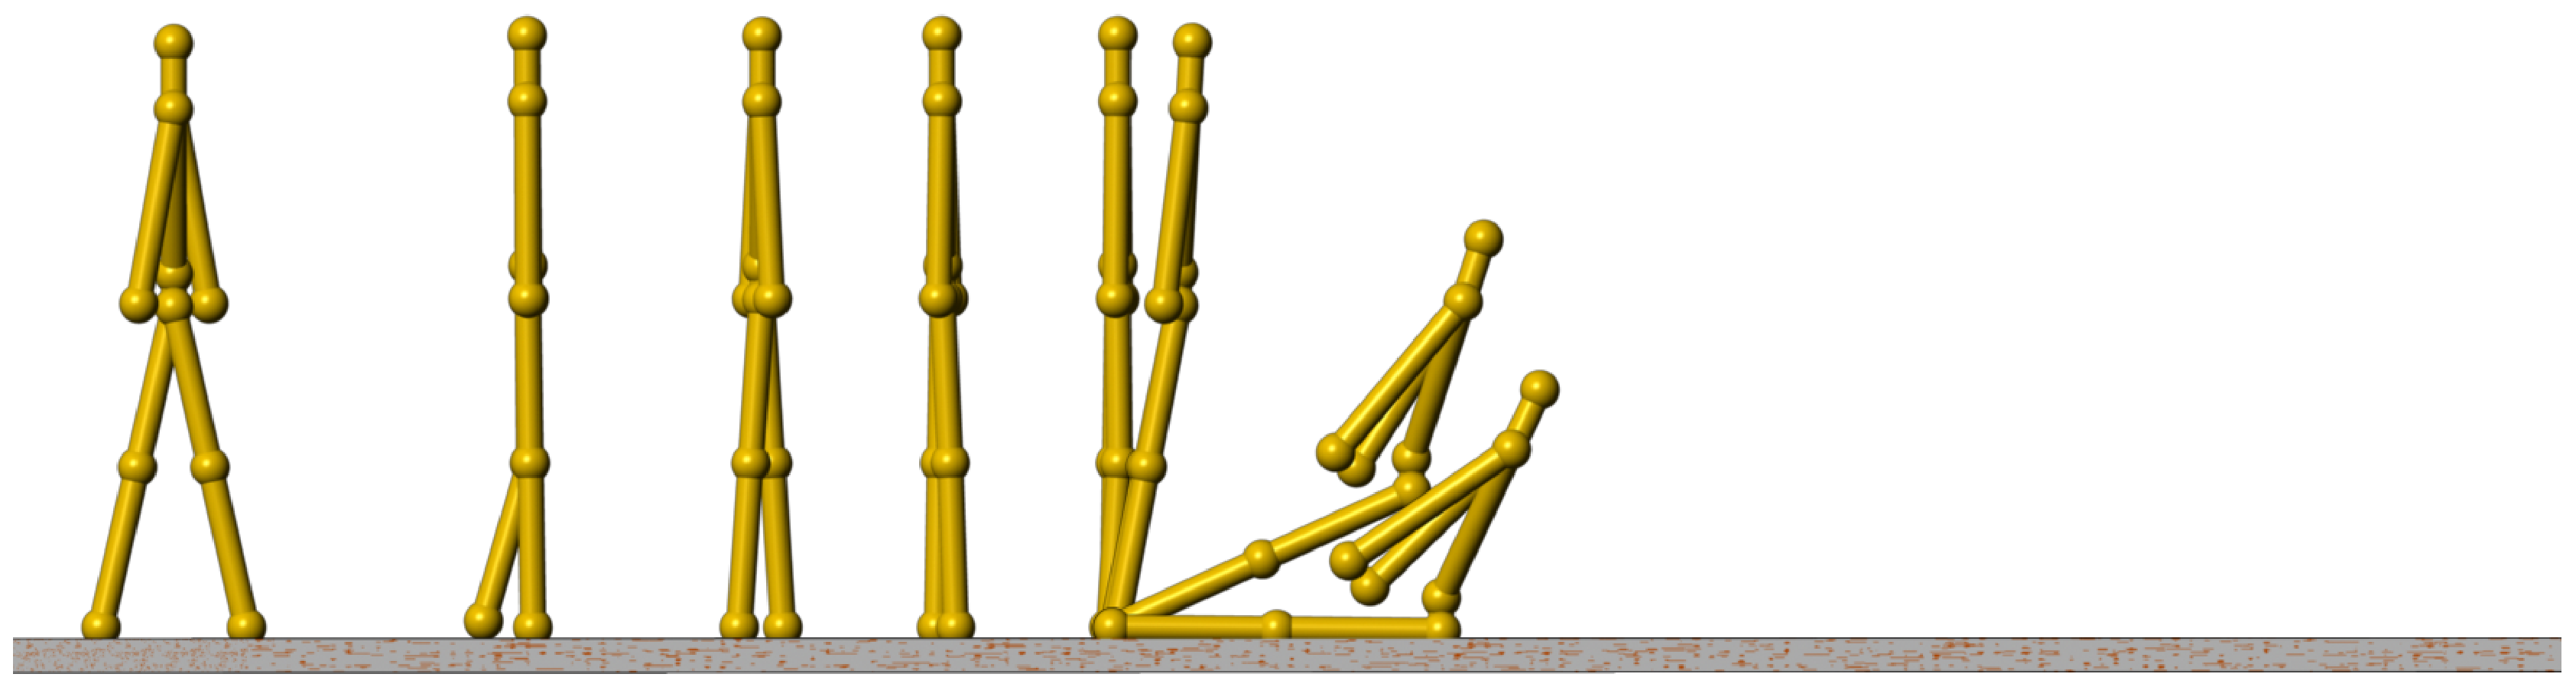
\includegraphics[height=6in]{PlaceHolder}
    \else
      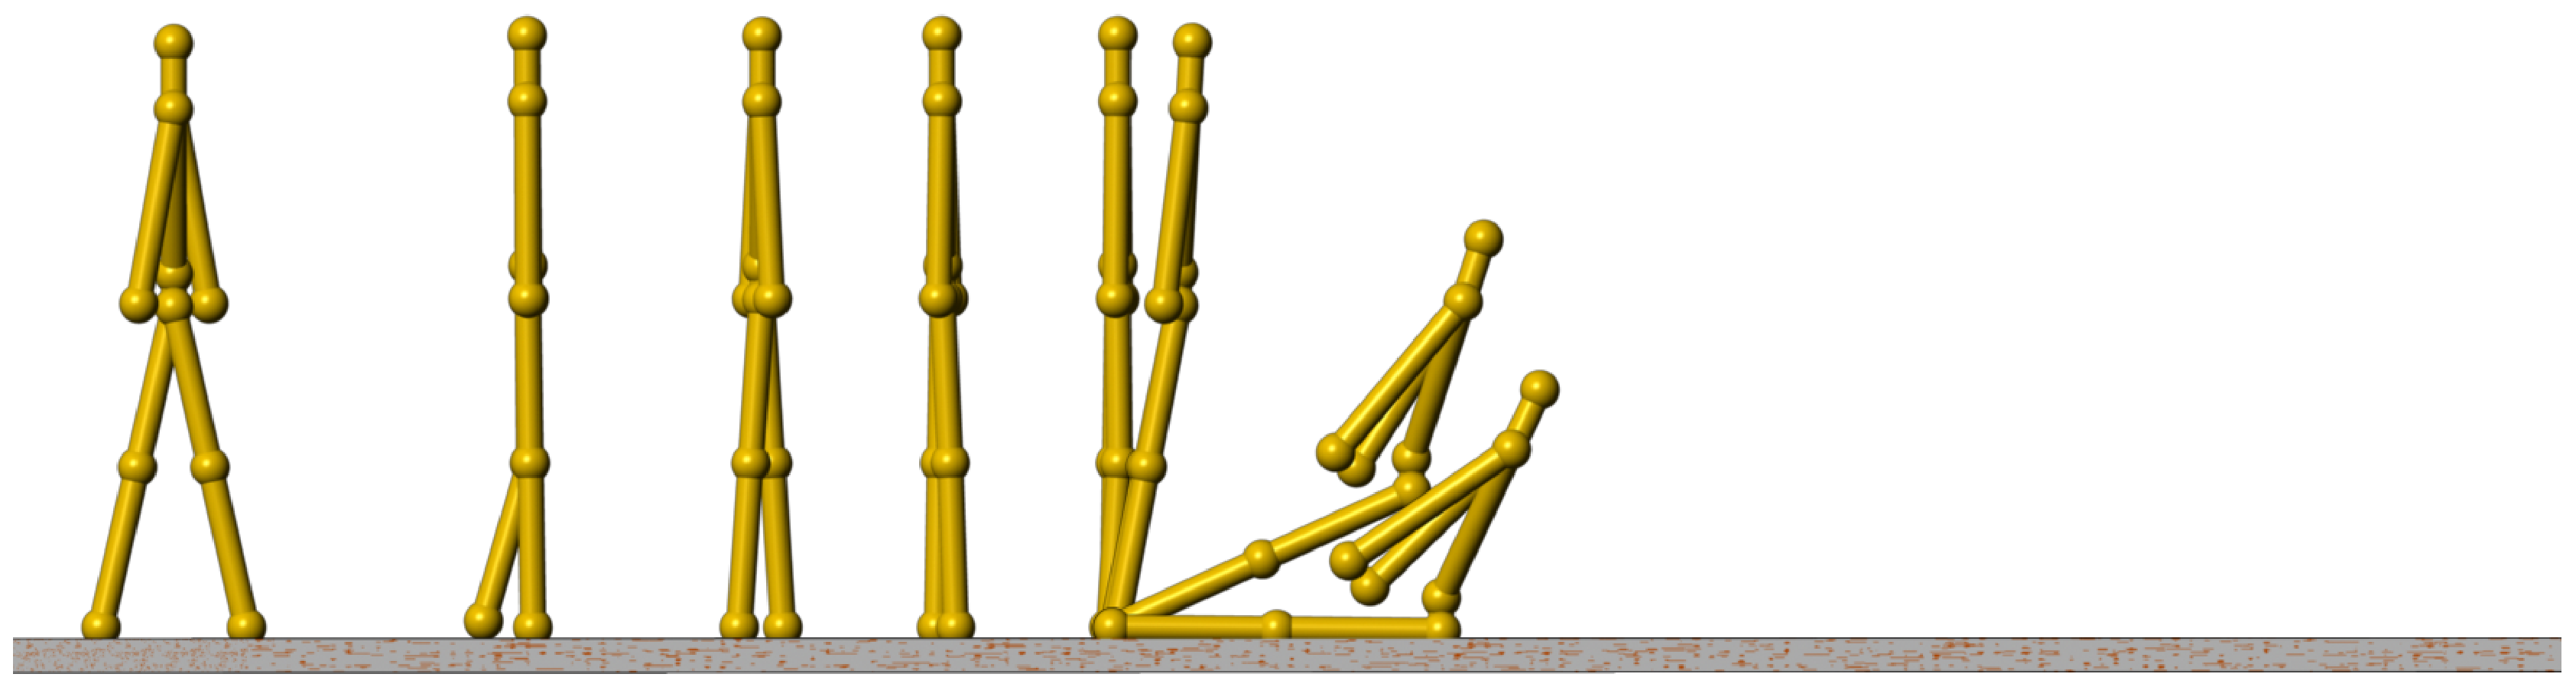
\includegraphics[width=0.7\textwidth]{PlaceHolder}
    \fi
    \caption{Place Holder}
    \label{fig:stancefall}
\end{center}
\end{figure}

\subsubsection*{Energy Control}
By modifying the Energy Scaling, we can modify the size of limit circle, the will adjust the oscillation amplitude.
as show in Figure~\ref{energyscaling}
\begin{figure}[!htbp]
  \begin{center}
    \leavevmode
    \ifpdf
      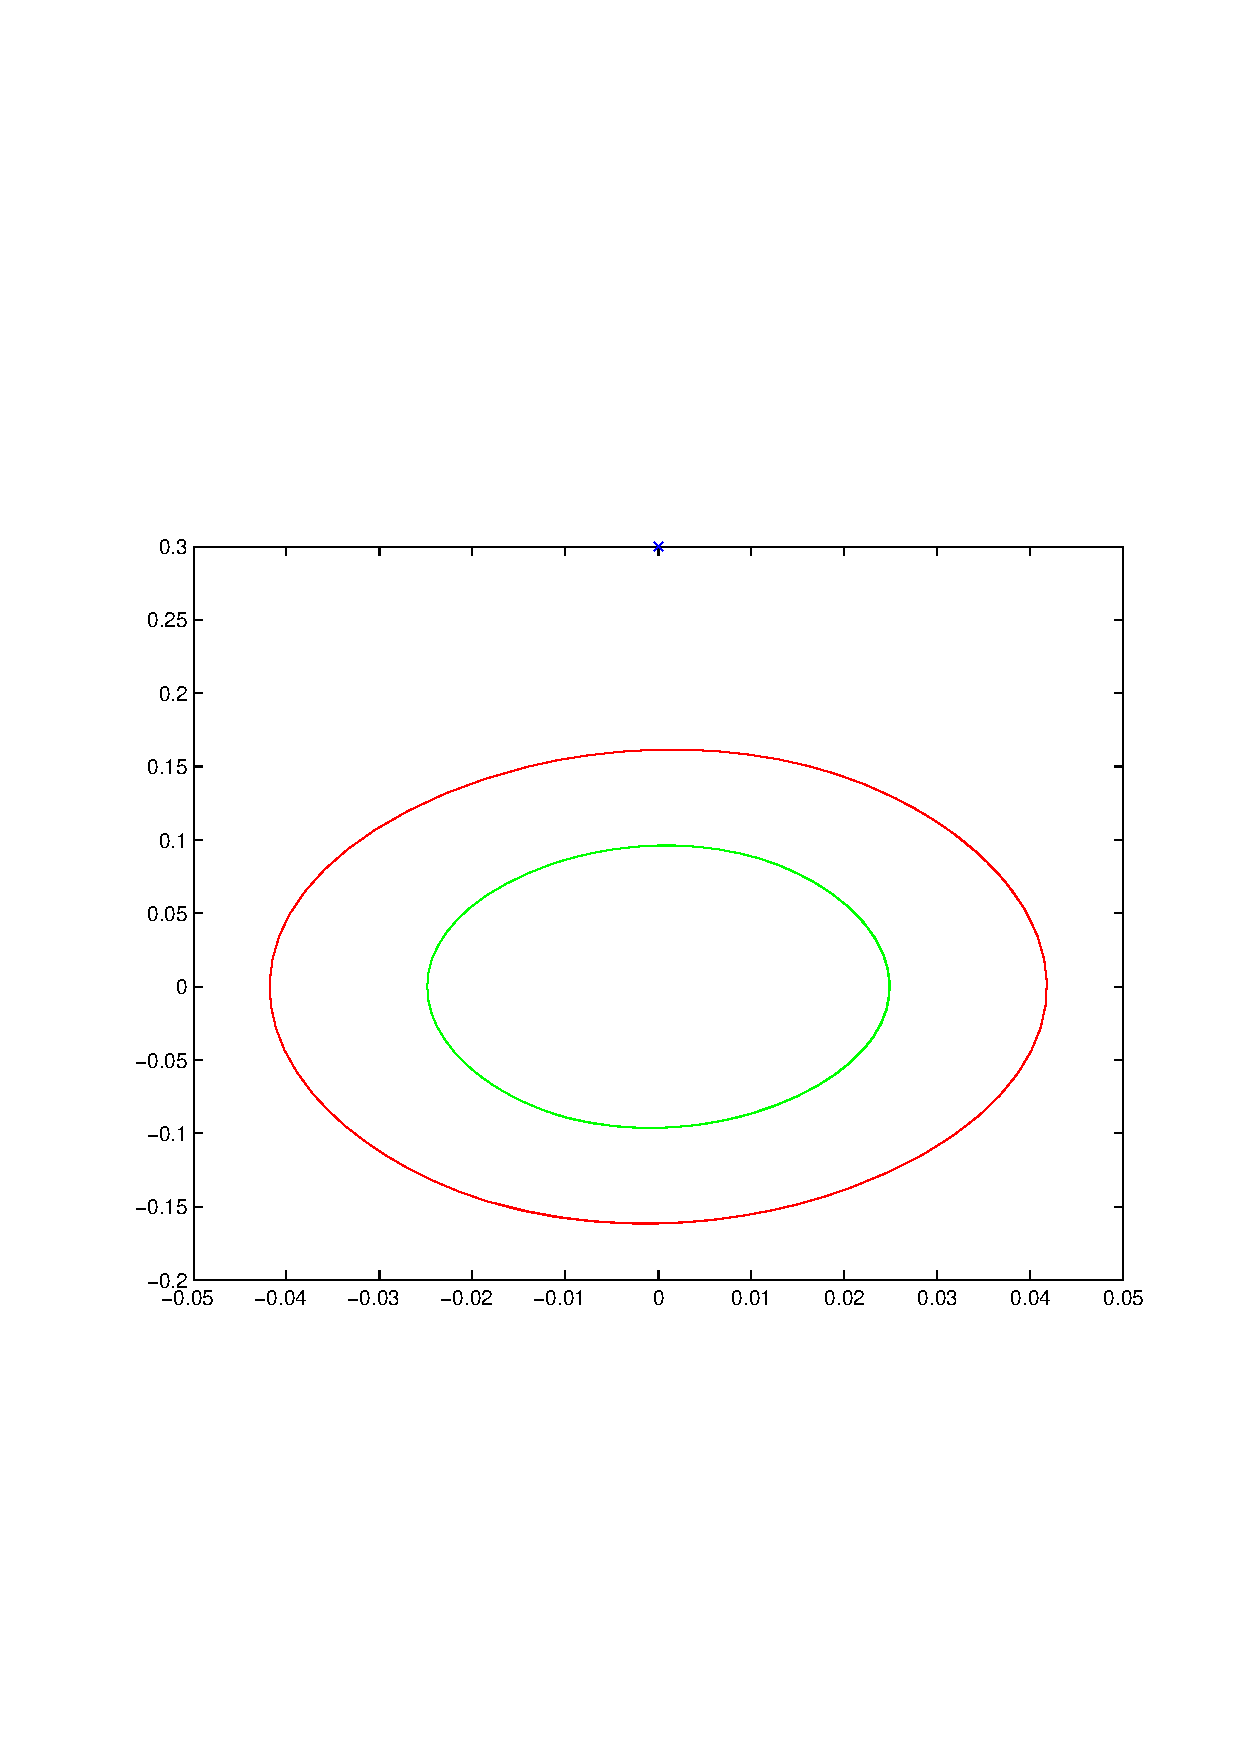
\includegraphics[height=6in]{EnergyControlled}
    \else
      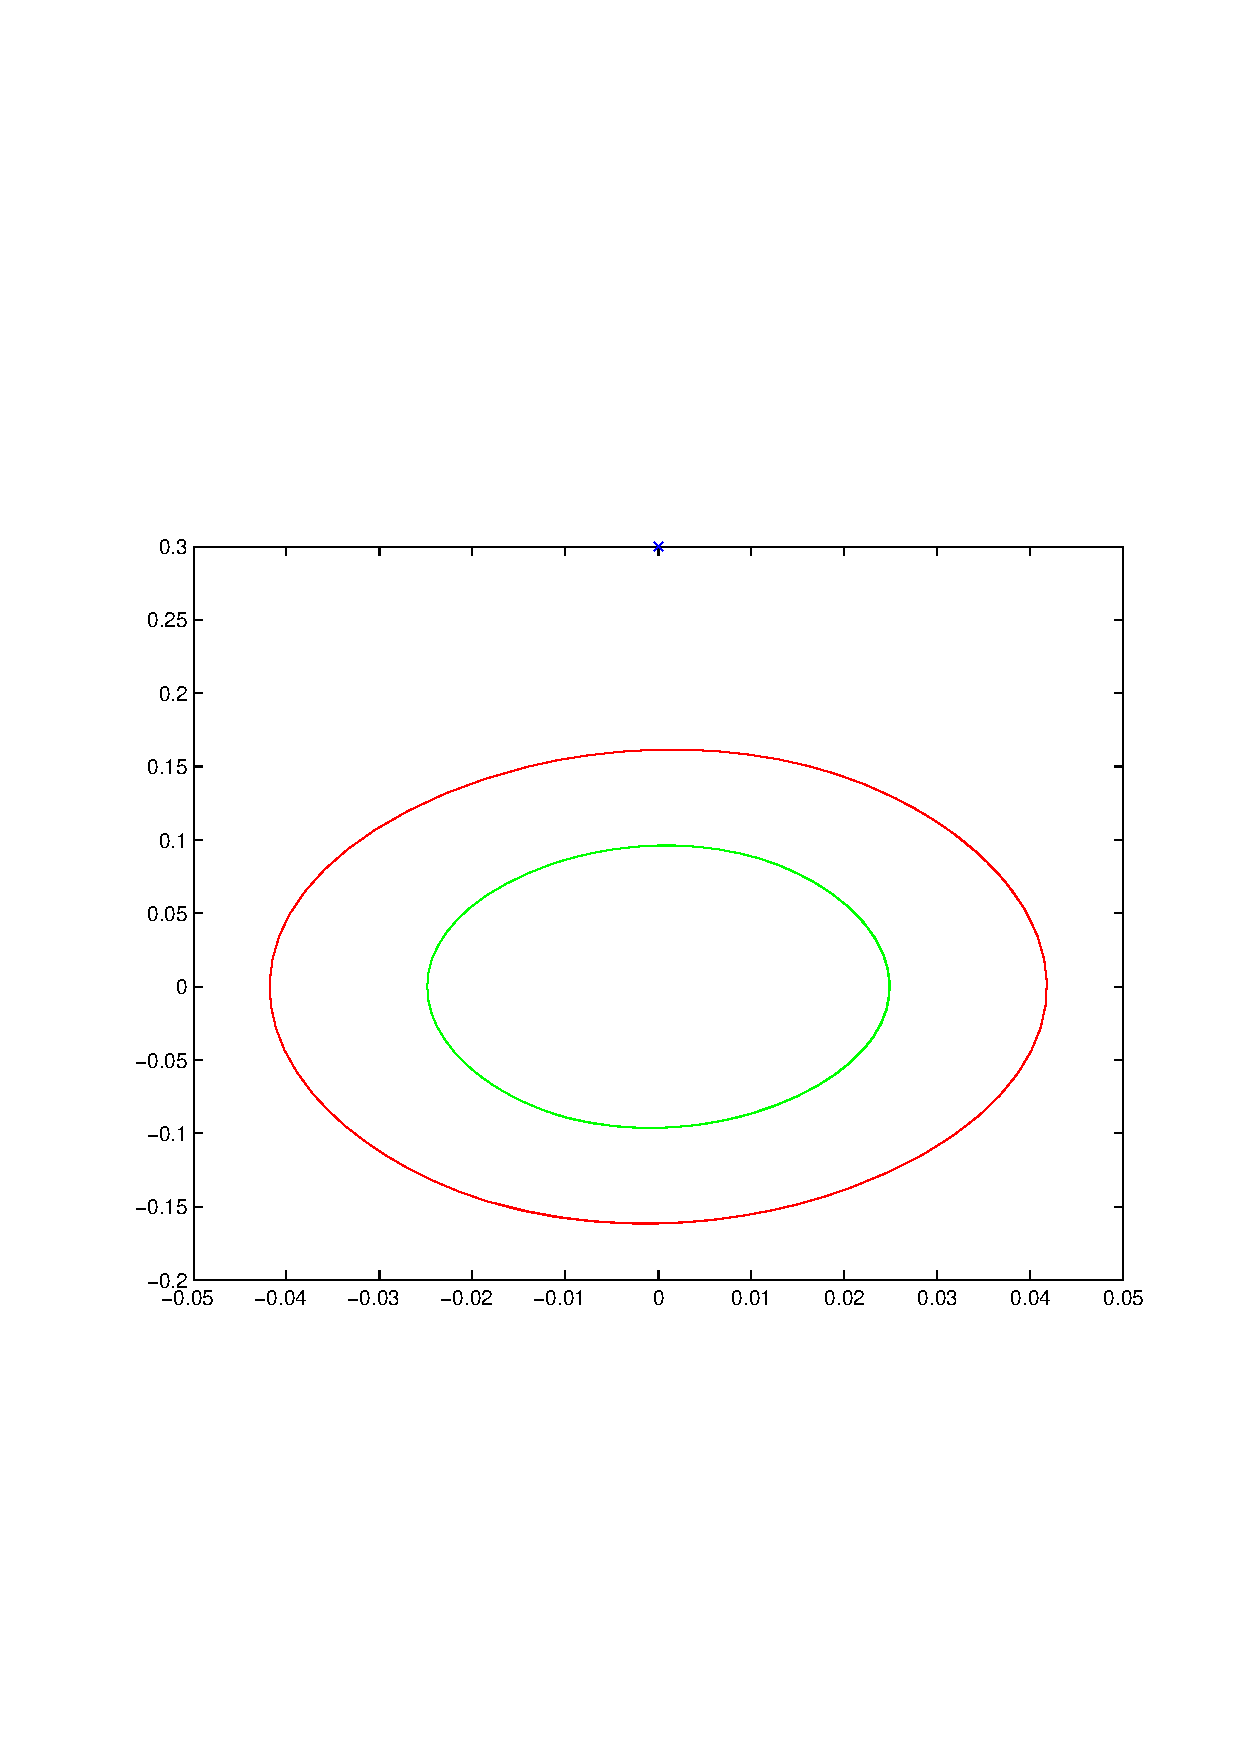
\includegraphics[width=0.7\textwidth]{EnergyControlled}
    \fi
    \caption{Energy Scaling}
    \label{fig:energyscaling}
\end{center}
\end{figure}

this will help the characters shrink the vibration amplitude.
but it will also shrink the size of basin of attraction.




\subsubsection*{Fast Stable}
by applying speed and energy scaling squarely, we can make the stance pos converge in a quick speed.
as shown in figure ~\ref{fig:fastconverg}
\begin{figure}[!htbp]
  \begin{center}
    \leavevmode
    \ifpdf
      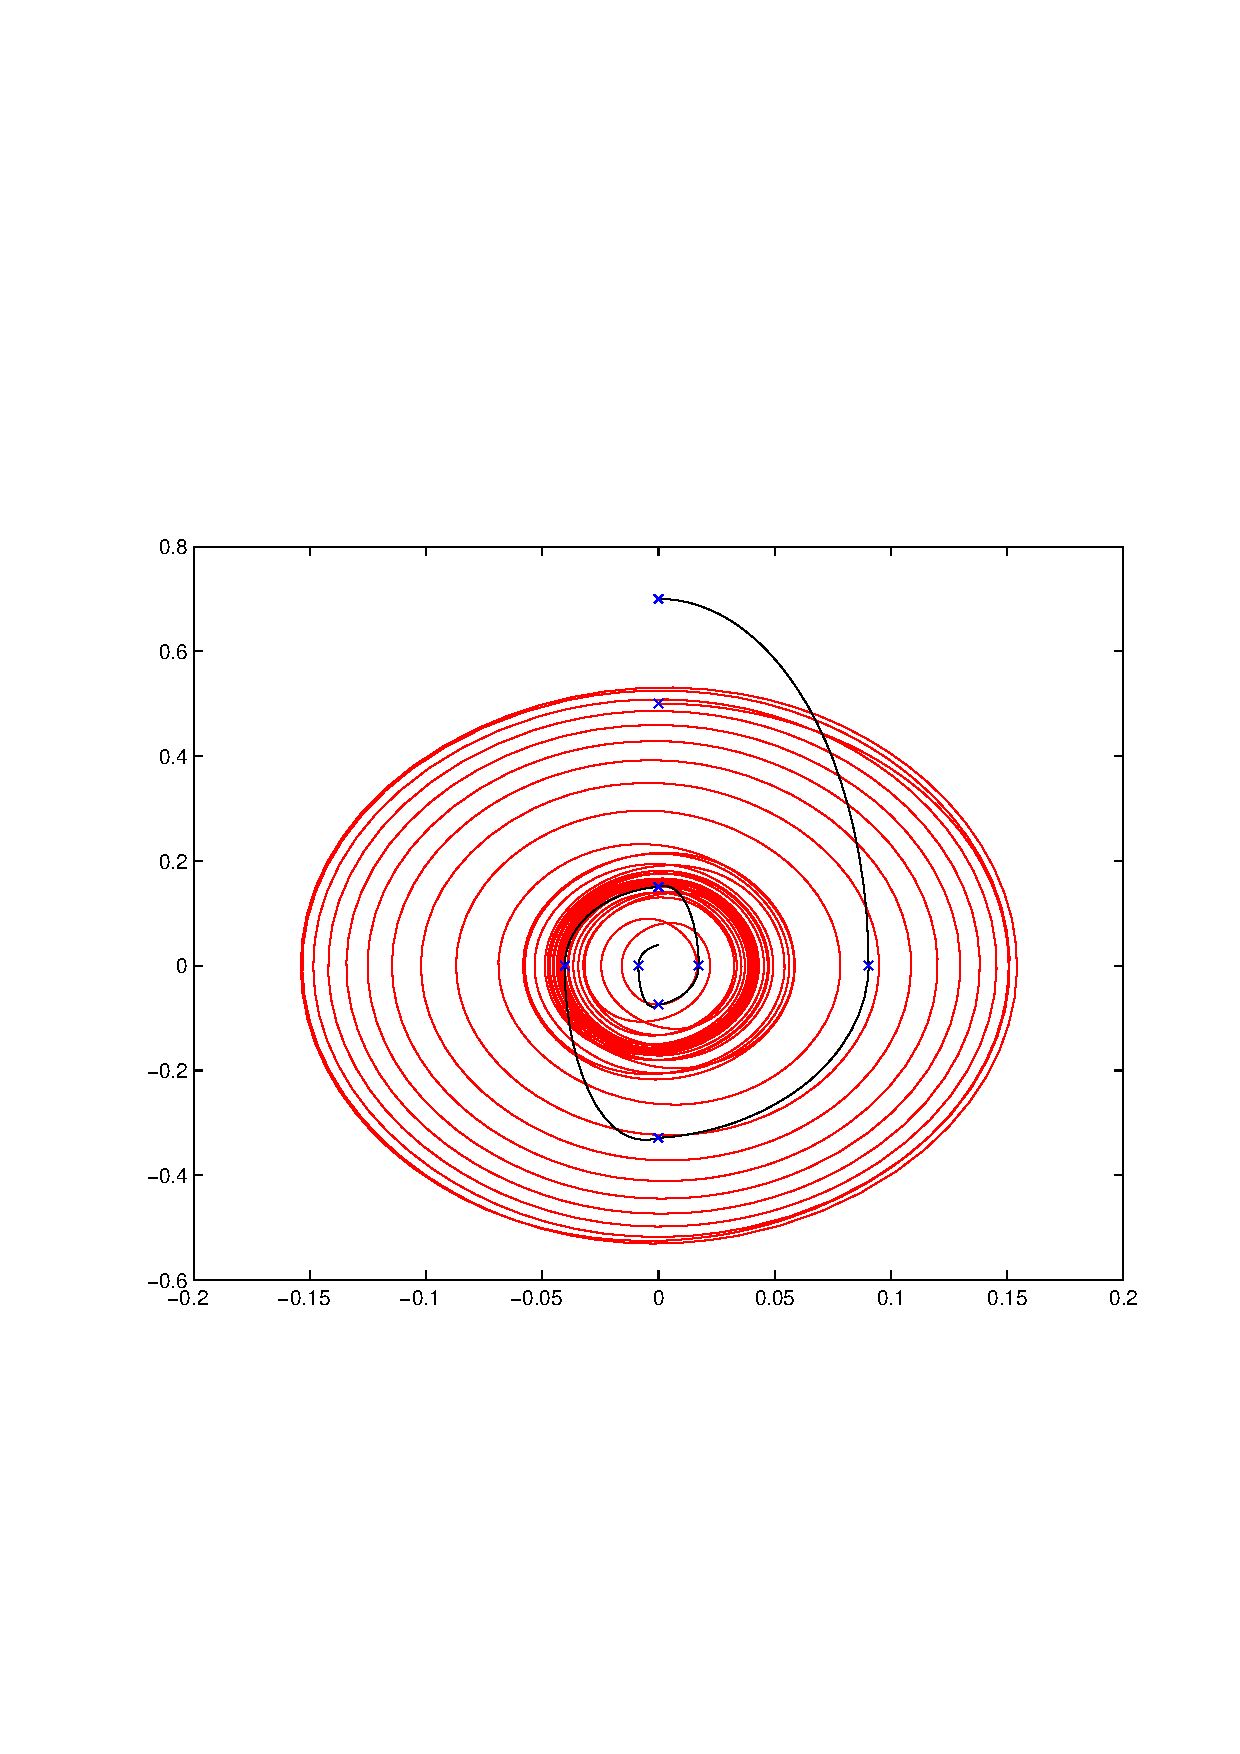
\includegraphics[height=6in]{FastCoverge}
    \else
      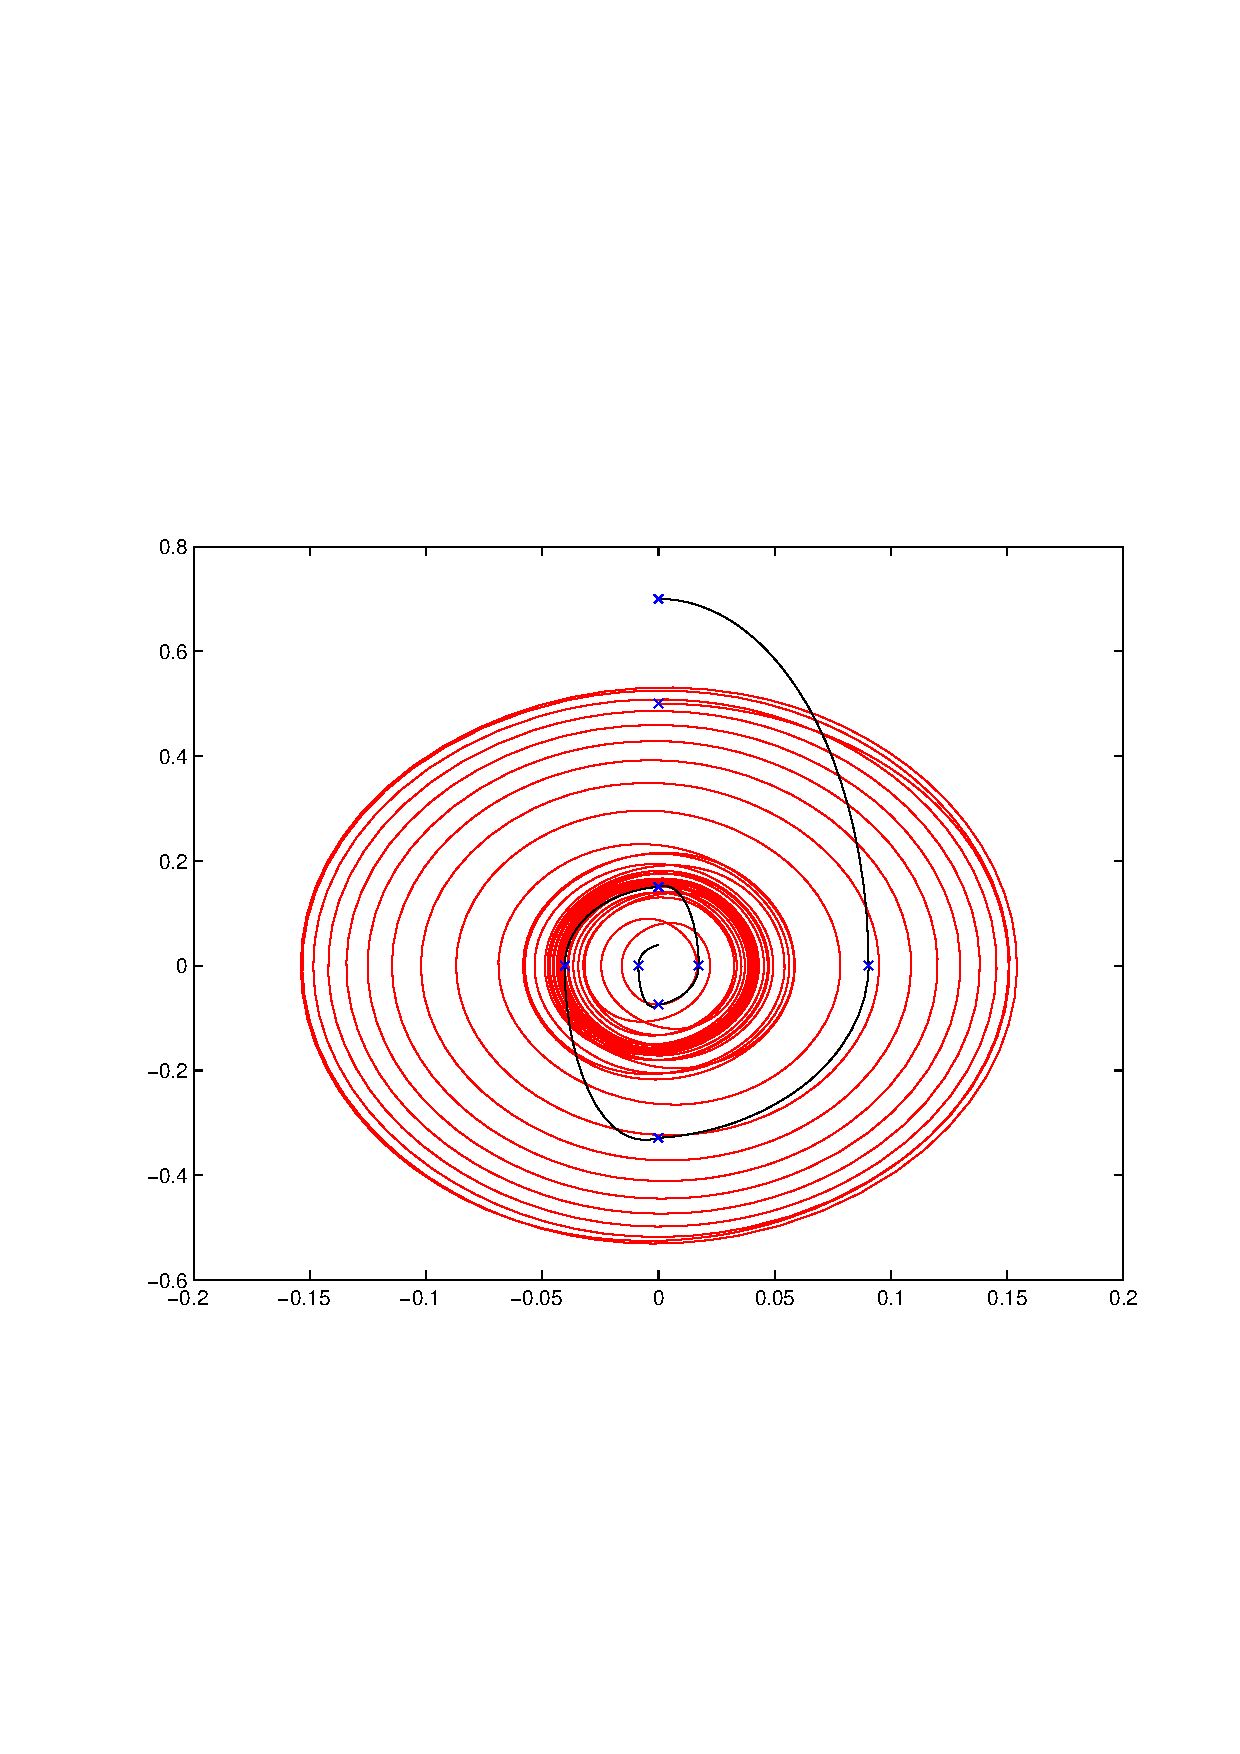
\includegraphics[width=0.7\textwidth]{FastCoverge}
    \fi
    \caption{Fast Converge}
    \label{fig:fastconverg}
\end{center}
\end{figure}


For comparation, we have three stance motion perturbed.
the left one is without any control and the characters fail.
the second one speed action is applied, characters maintain its stance motion, but vibrate.
the third is both speed action and energy action are applied, the character maintain the stance and also vibrate with shrinking amplitude.

\begin{figure}[!htbp]
  \begin{center}
    \leavevmode
    \ifpdf
      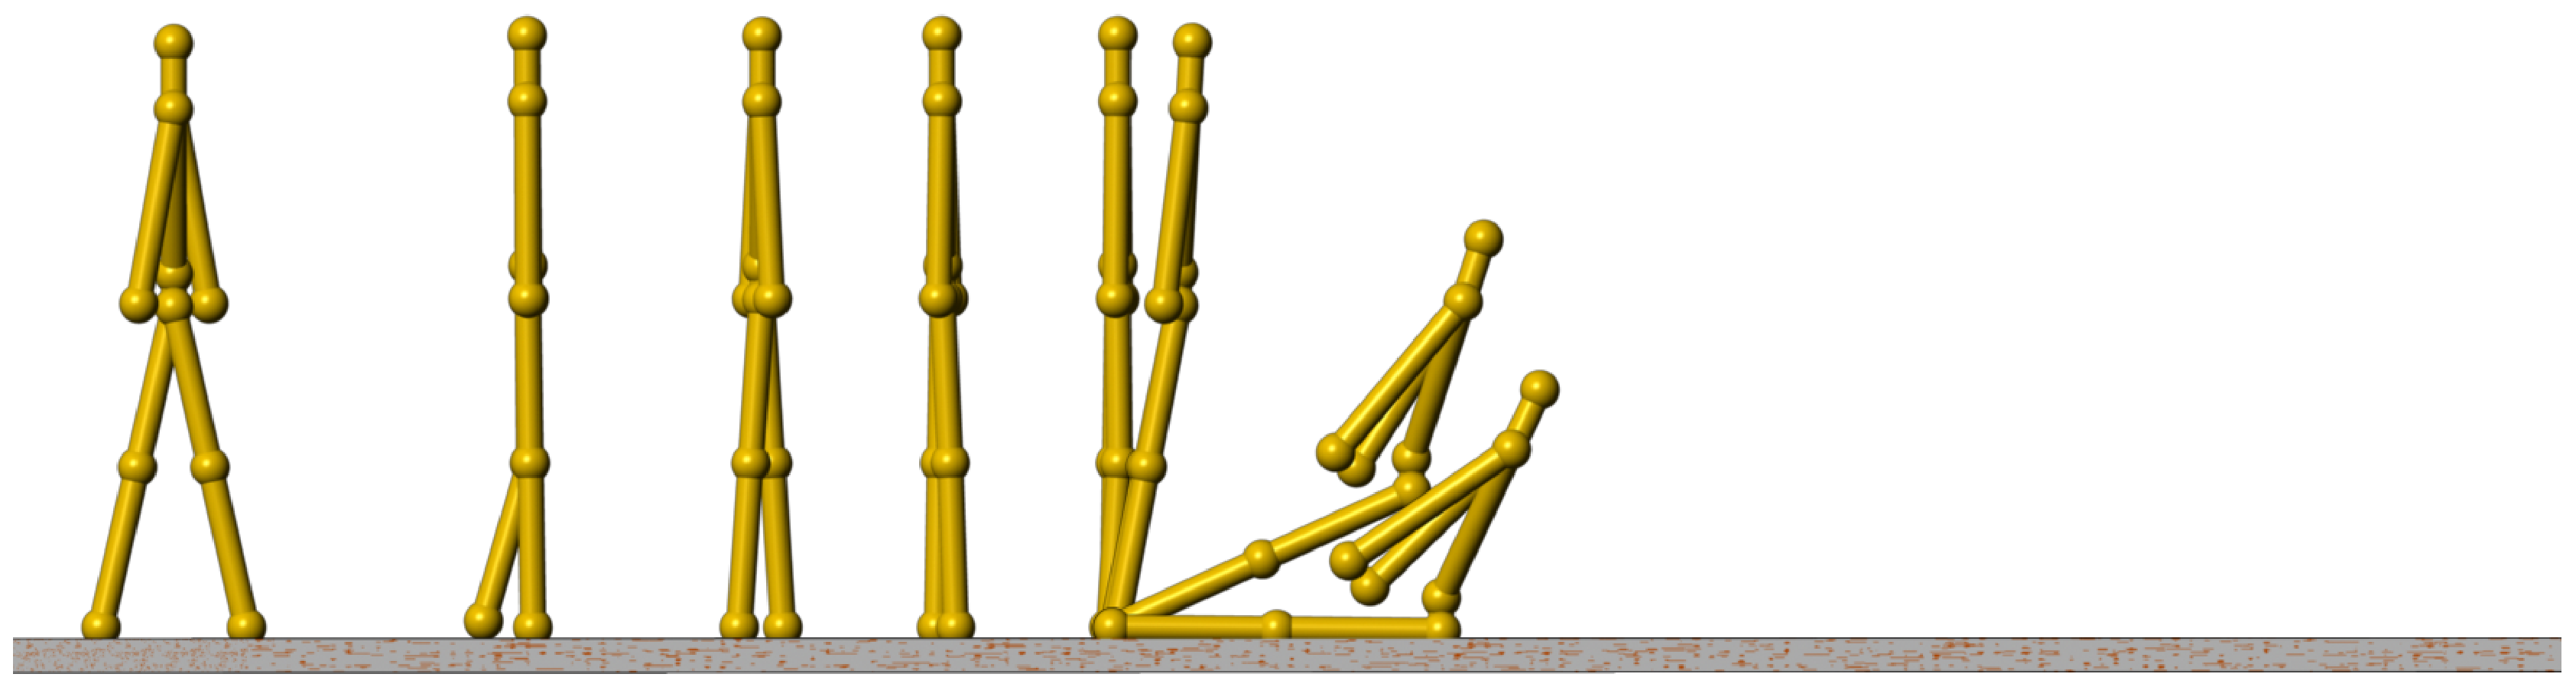
\includegraphics[height=6in]{PlaceHolder}
    \else
      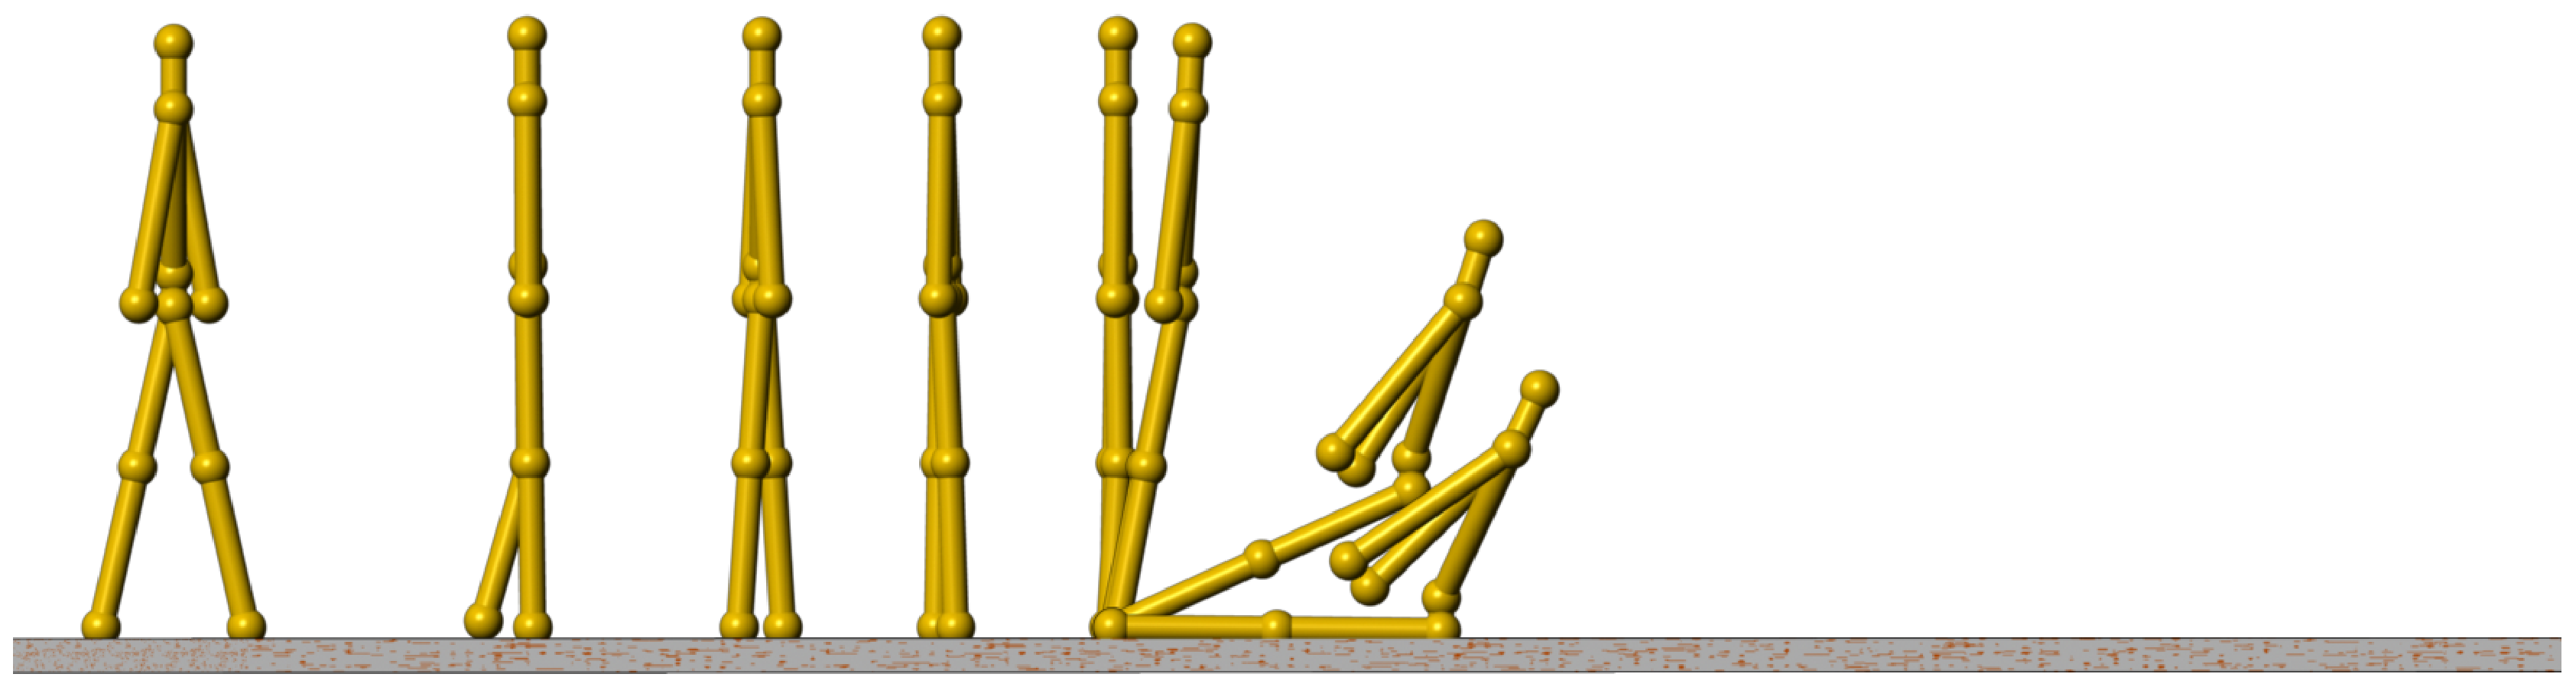
\includegraphics[width=0.7\textwidth]{PlaceHolder}
    \fi
    \caption{Place Holder1}
    \label{fig:stancefall}
\end{center}
\end{figure}

\begin{figure}[!htbp]
  \begin{center}
    \leavevmode
    \ifpdf
      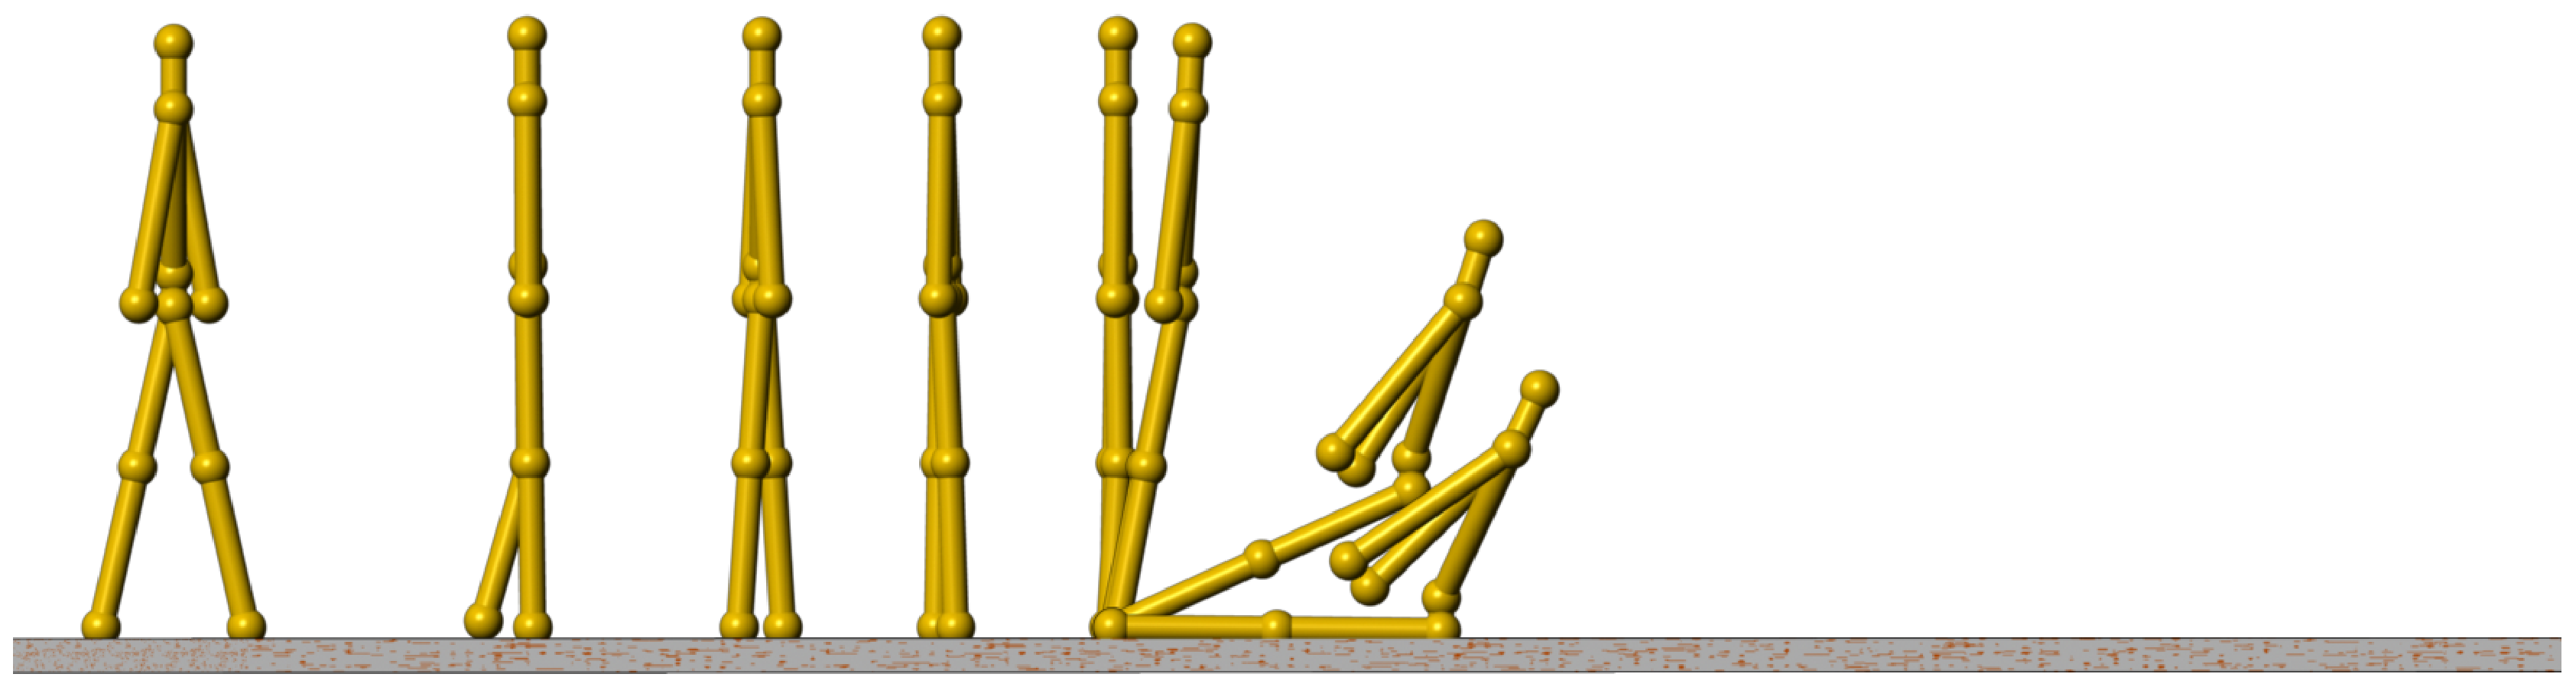
\includegraphics[height=6in]{PlaceHolder}
    \else
      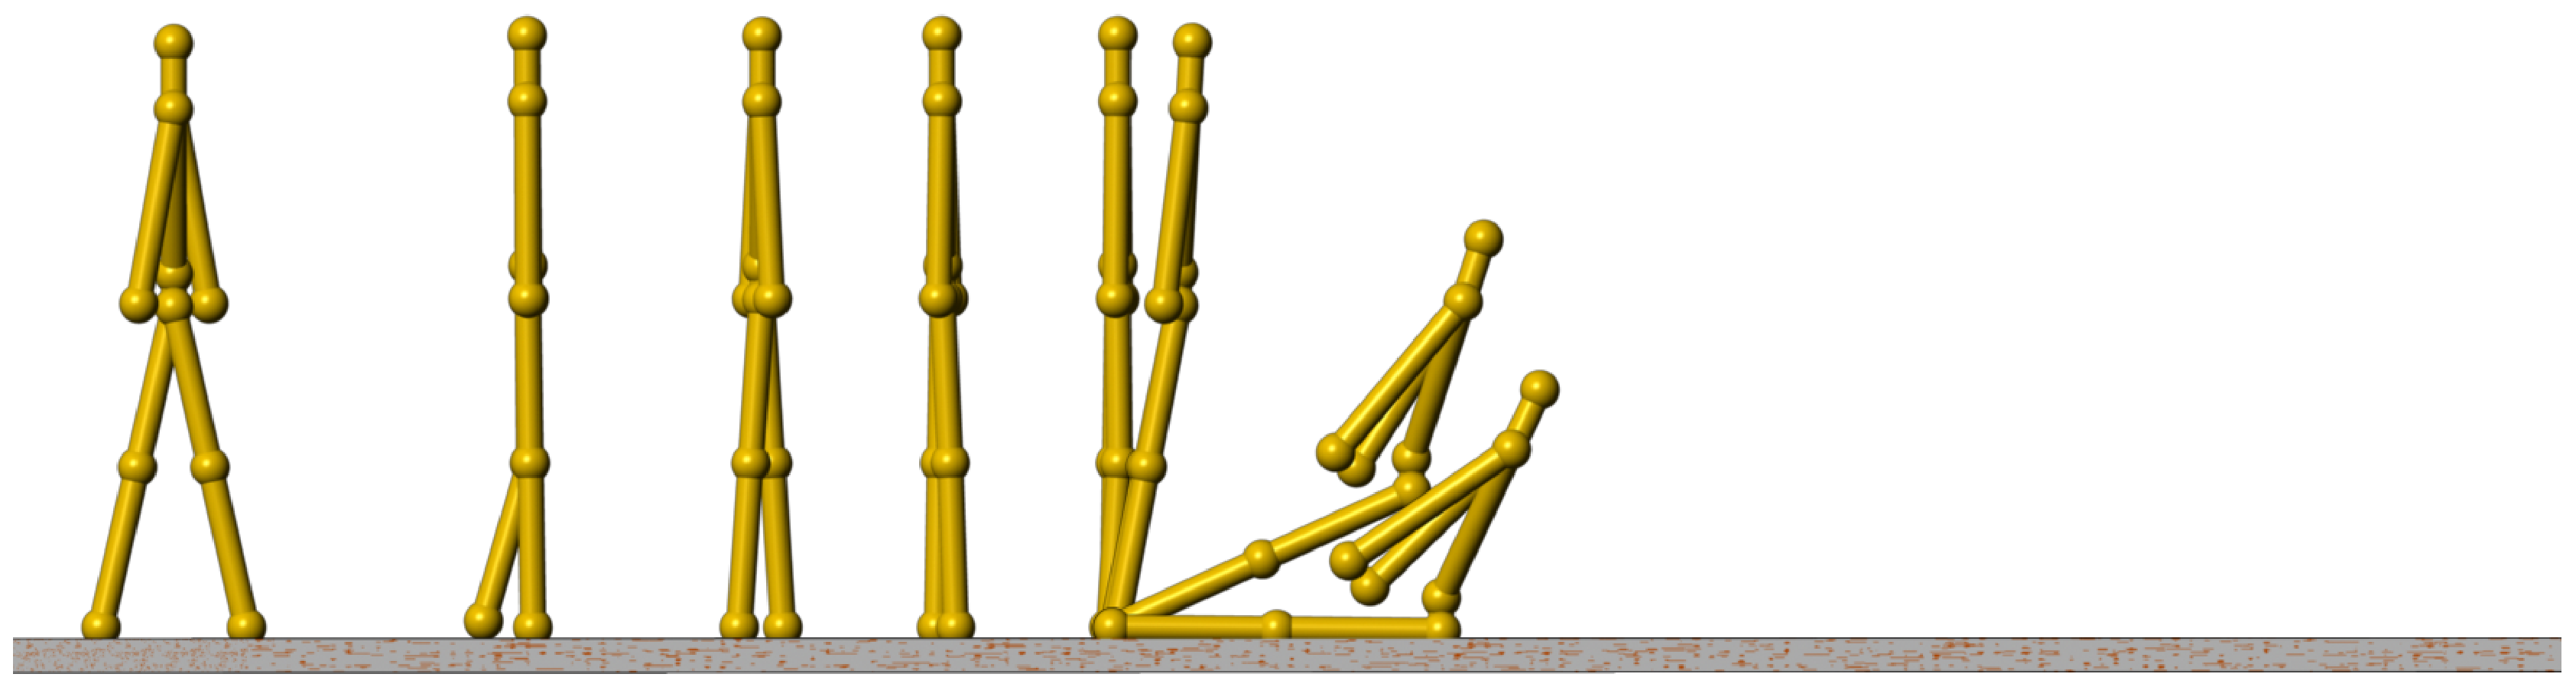
\includegraphics[width=0.7\textwidth]{PlaceHolder}
    \fi
    \caption{Place Holder1}
    \label{fig:stancefall}
\end{center}
\end{figure}



\section{Walking and Stance Transition}
we phase plot we show the limit circle of two motion primitives.

\begin{figure}[!htbp]
  \begin{center}
    \leavevmode
    \ifpdf
      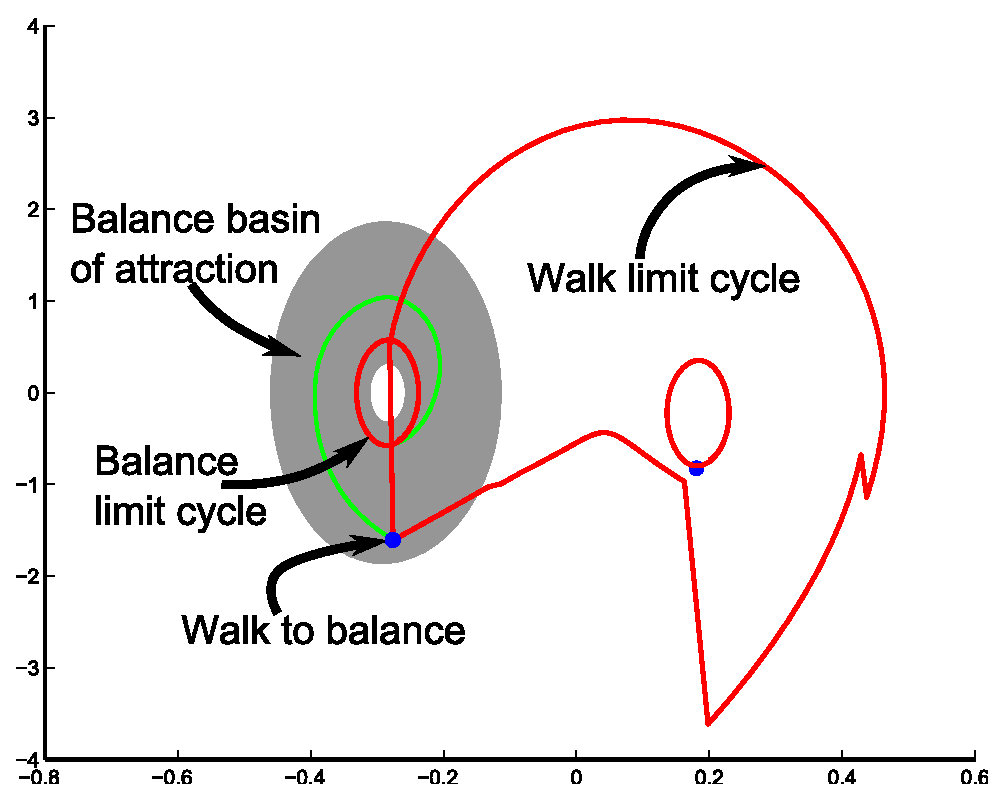
\includegraphics[height=6in]{walk_to_stand}
    \else
      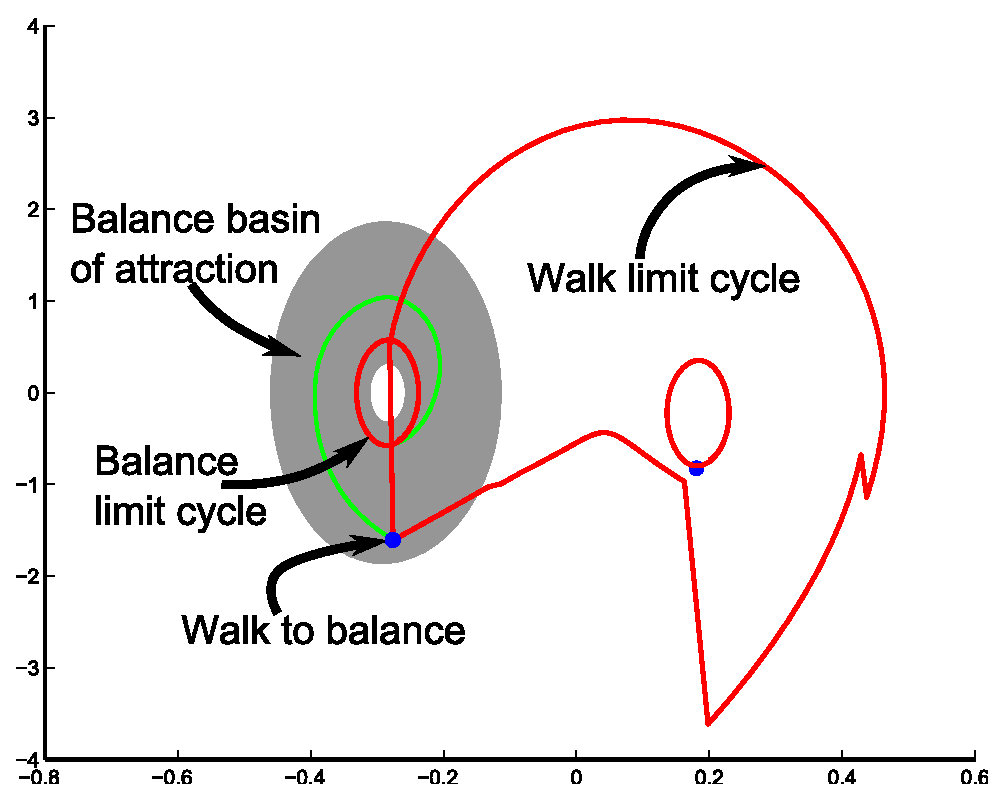
\includegraphics[width=0.7\textwidth]{walk_to_stand}
    \fi
    \caption{Fast Converge}
    \label{fig:fastconverg}
\end{center}
\end{figure}

the phase plot here shows the supporting leg, the swing leg is show in shadow red


\subsection{Walk to Stance}
walk to stance transition happens at the heel strike phase.
if without control effort, the bipedal machine will continue two walk, while if we switch the on the stance controller,
the bipedal machine will converge to a small amplitue,then both legs start oscillation, this is the stance to walk.

we show in picture
\begin{figure}[!htbp]
  \begin{center}
    \leavevmode
    \ifpdf
      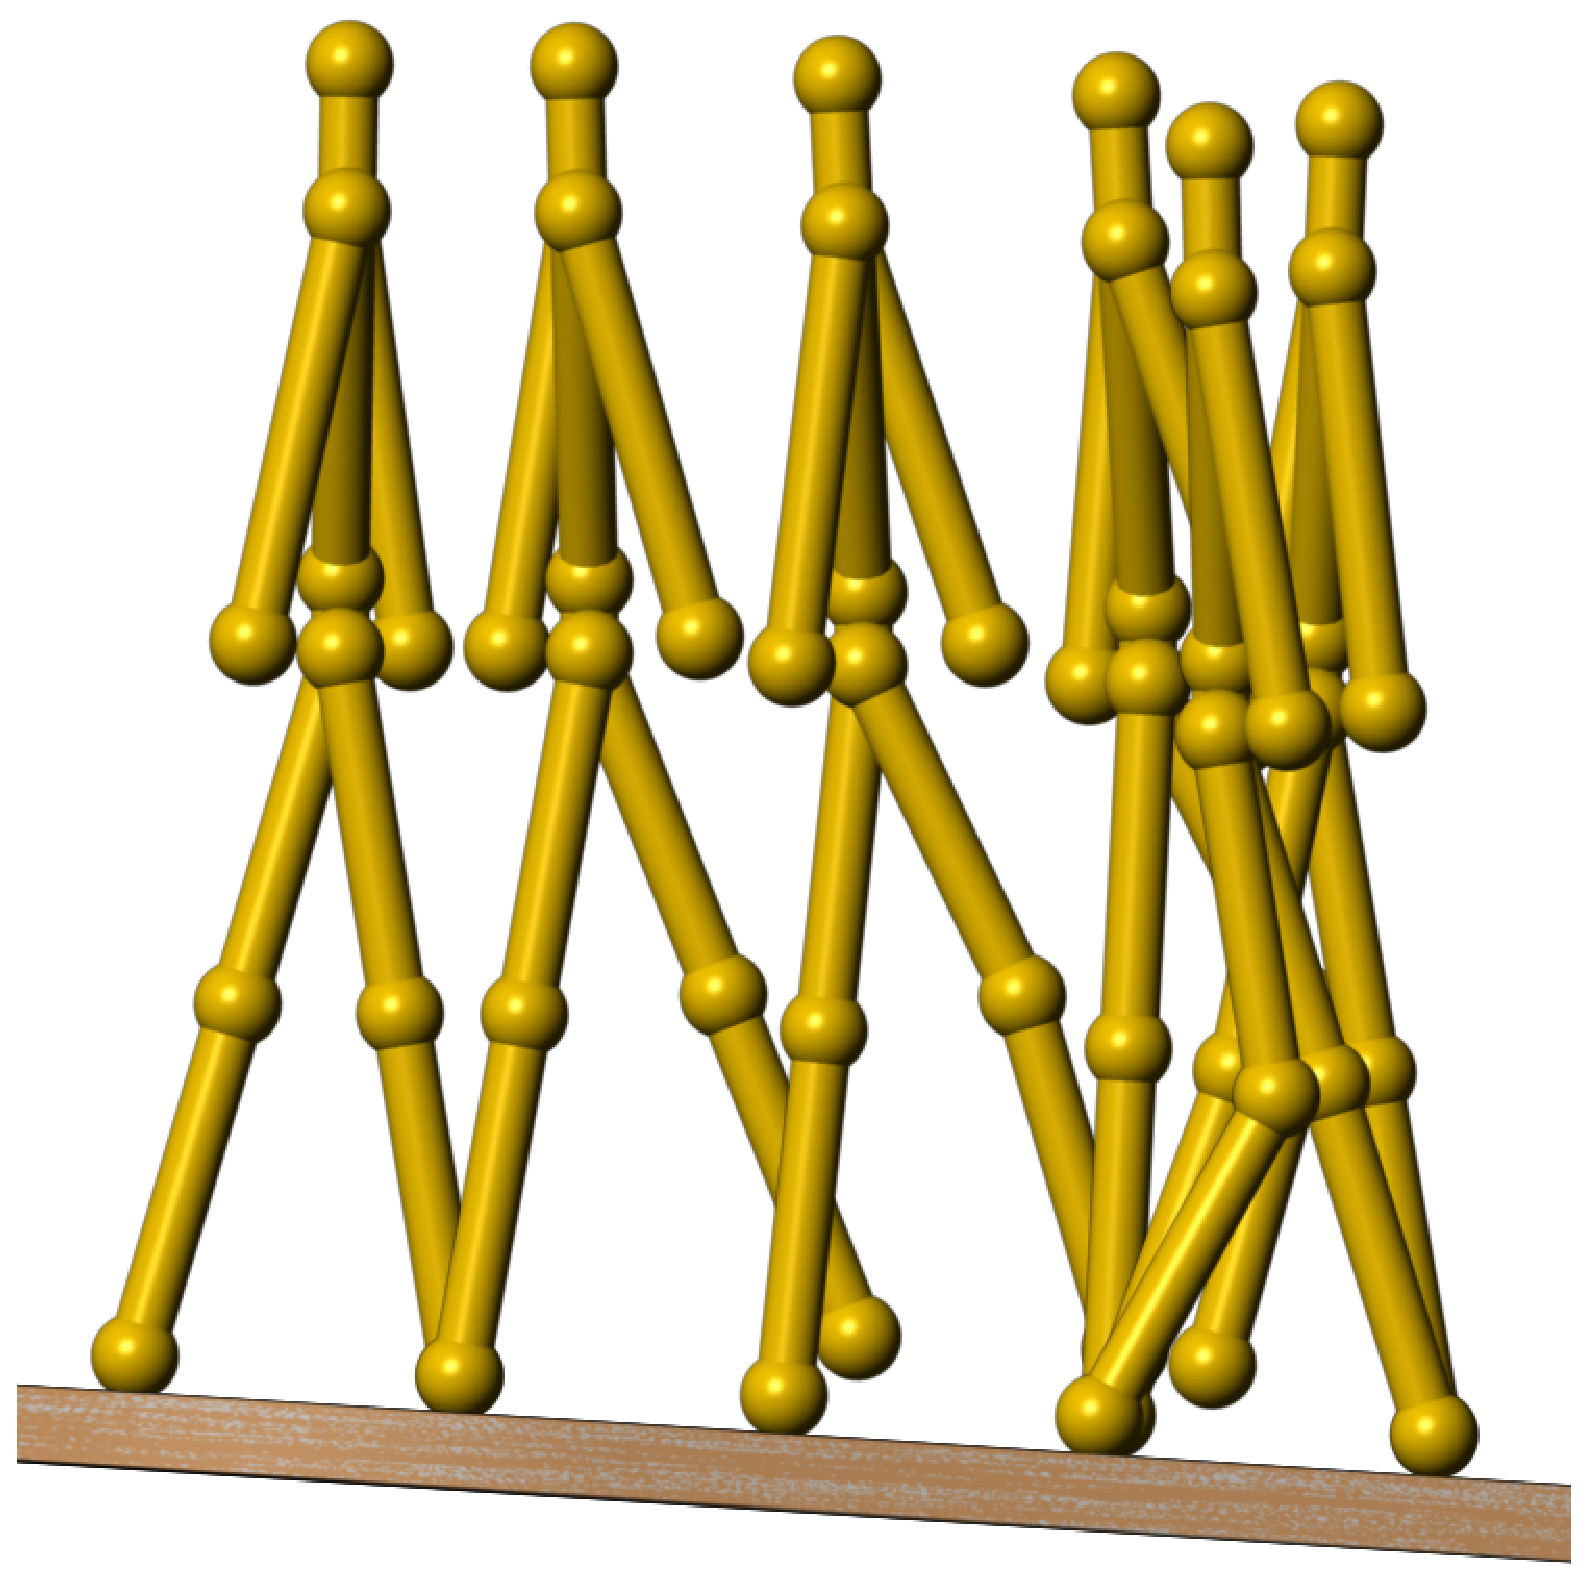
\includegraphics[height=6in]{walk_to_balance}
    \else
      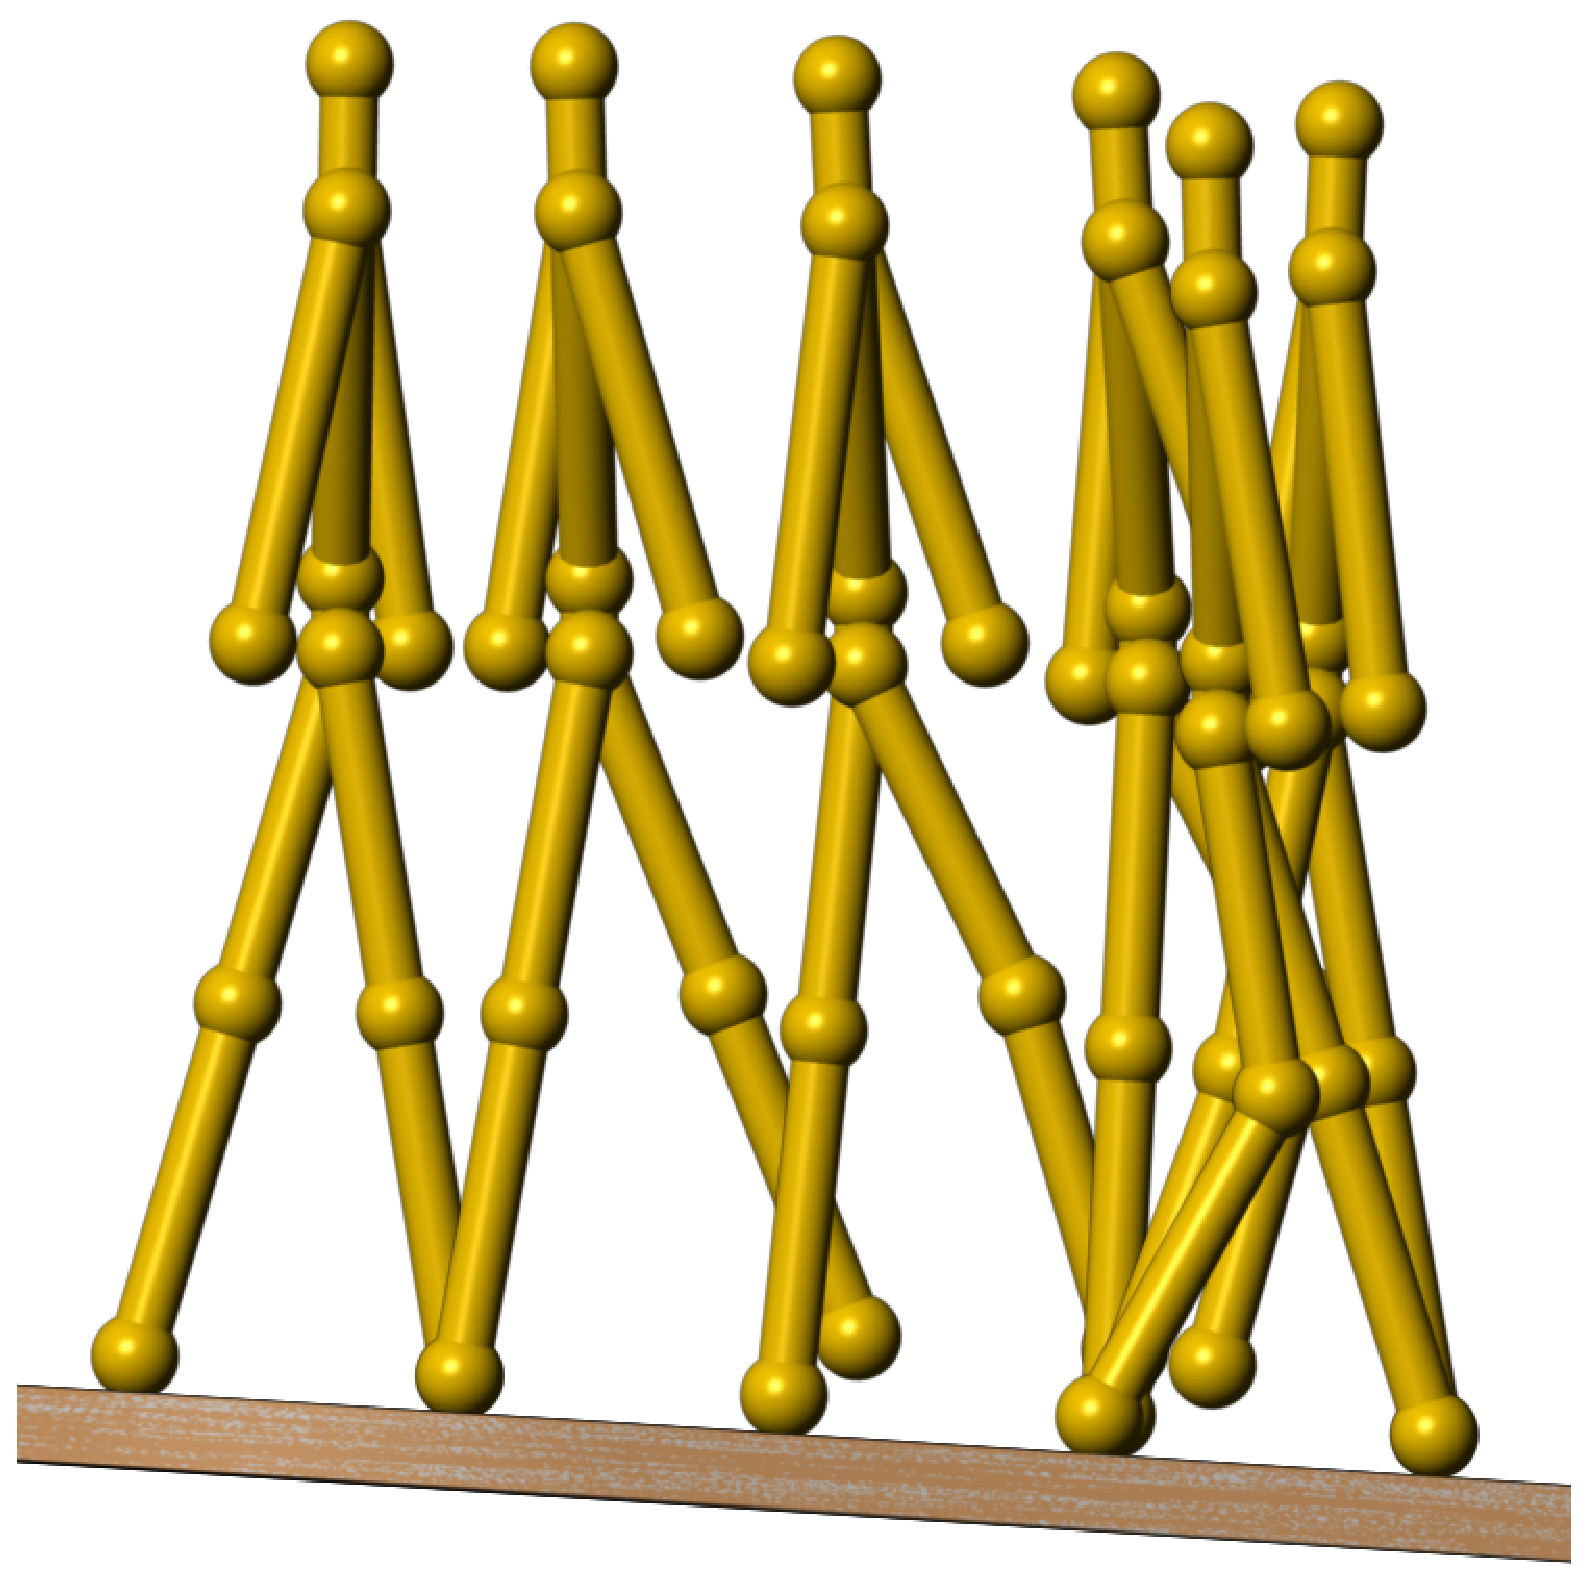
\includegraphics[width=0.7\textwidth]{walk_to_balance}
    \fi
    \caption{Walk to Balance}
    \label{fig:walk to balance}
\end{center}
\end{figure}

When walk to stance happens, the walker have to the stance controller must include the heel strike position.


\subsubsection*{Knee Bending Scheme}
When from walk to stance, that the heel strike time, the two legs are straight, for this case, the support region is very small.
Any push of the figure, it will move out of the two support region.
the walkers have to bend legs and lower the height.
Many possible ways can be develop for bending to lower the body height
We have develop many bending scheme, have seen many possible usage of the bending

\begin{itemize}
	\HiItem{One Leg Bending}
		walker can bend one leg while keep the other leg straight.
	\HiItem{Double Leg Bending}
		We can make the two leg bend.
\end{itemize}

it is very difficult to tell which one more realistic for human, basically, for when human walk, the knees is not necessary straight.
two schemes provide is the lexeme condition.

we have walking stance transition is shown in the following figures

\begin{figure}[!htbp]
  \begin{center}
    \leavevmode
    \ifpdf
      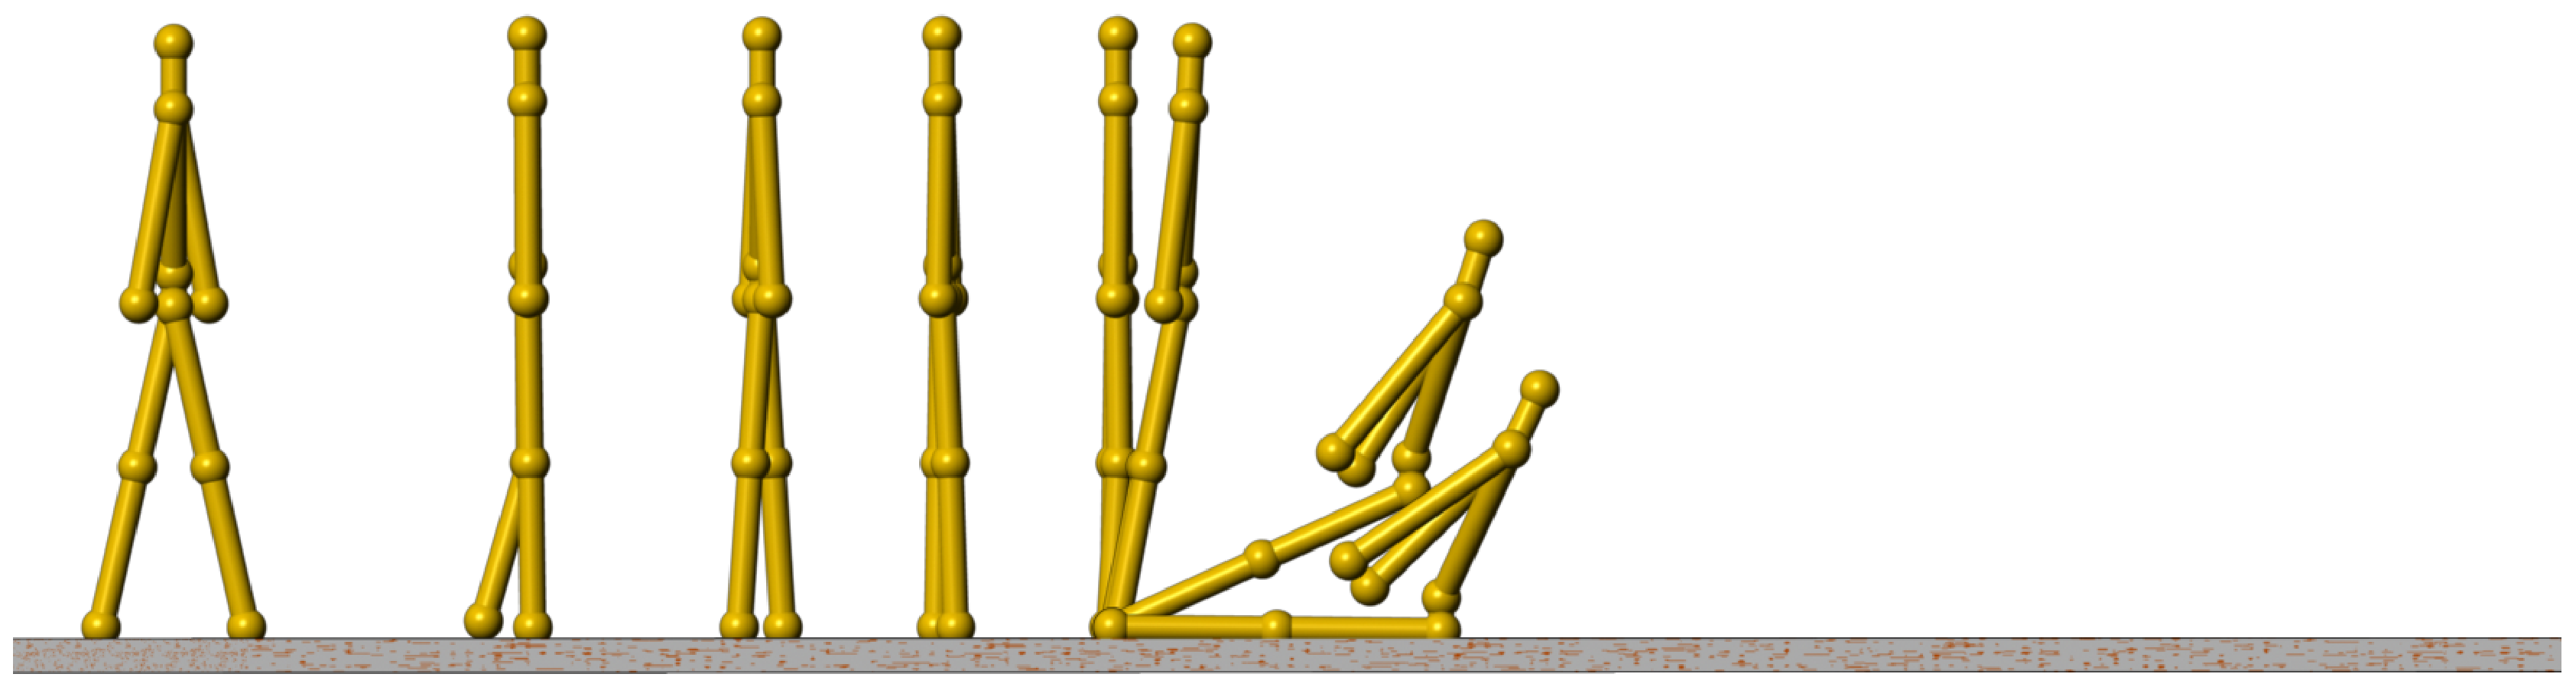
\includegraphics[height=6in]{PlaceHolder}
    \else
      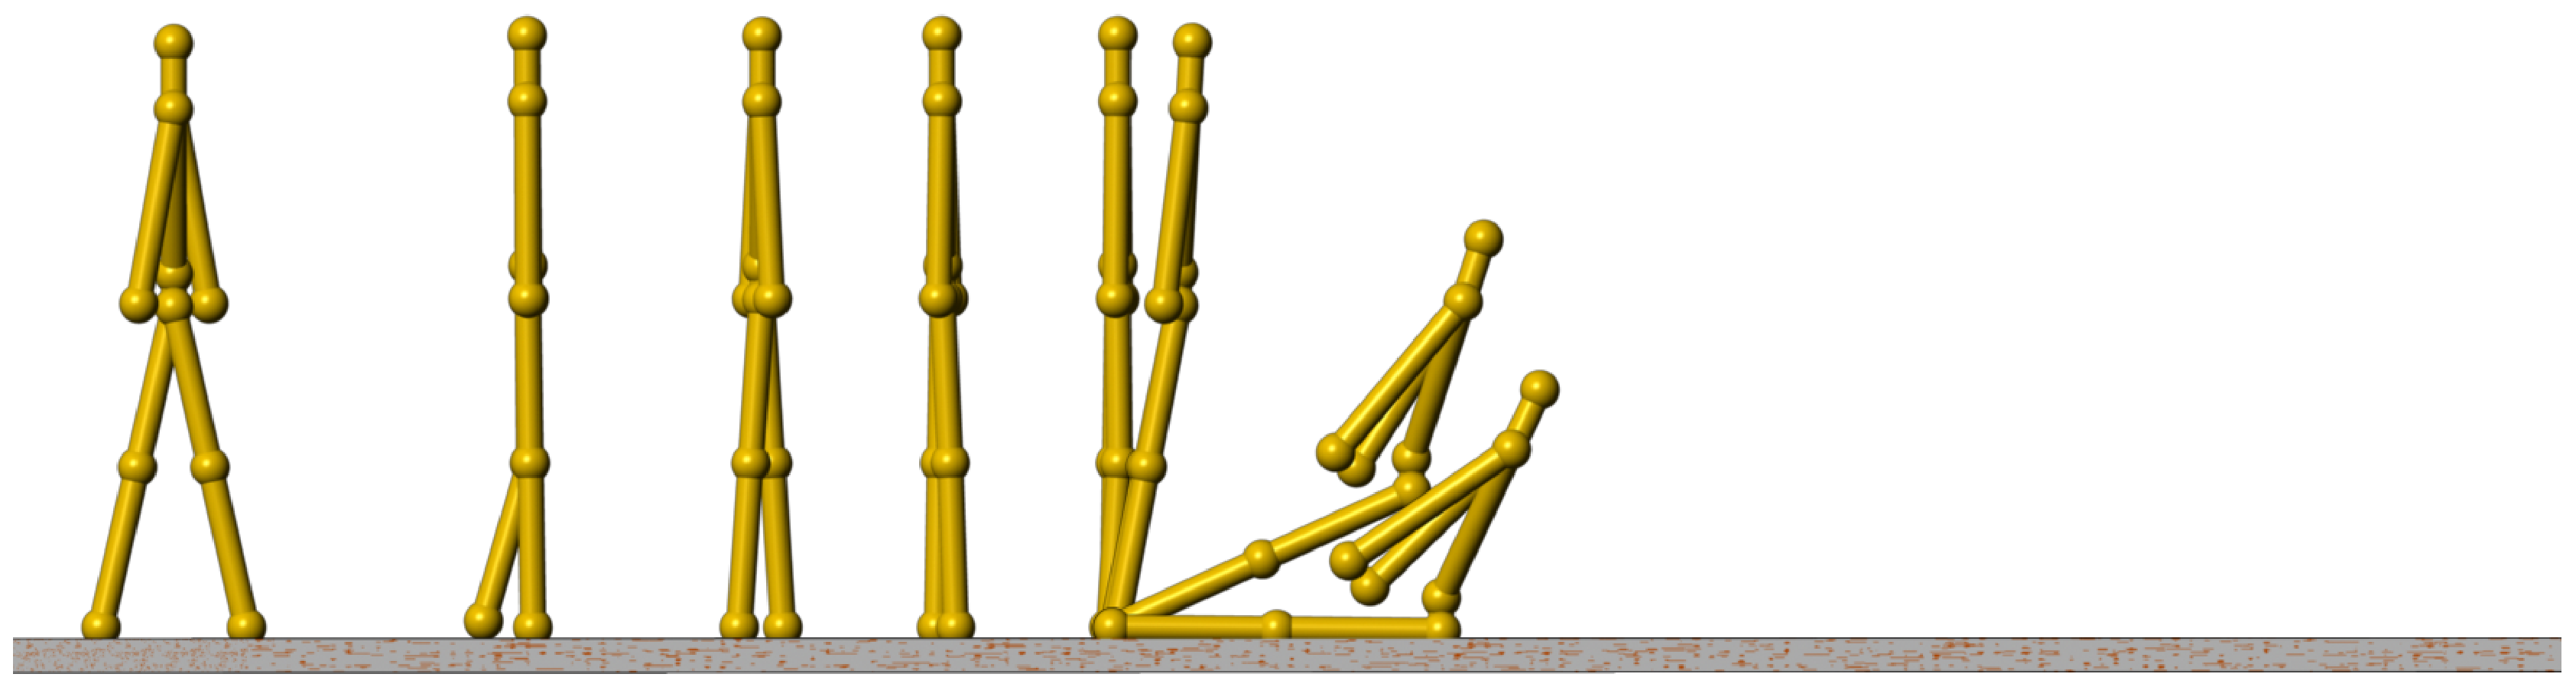
\includegraphics[width=0.7\textwidth]{PlaceHolder}
    \fi
    \caption{Place Holder}
    \label{fig:walkstancestraight}
\end{center}
\end{figure}

\begin{figure}[!htbp]
  \begin{center}
    \leavevmode
    \ifpdf
      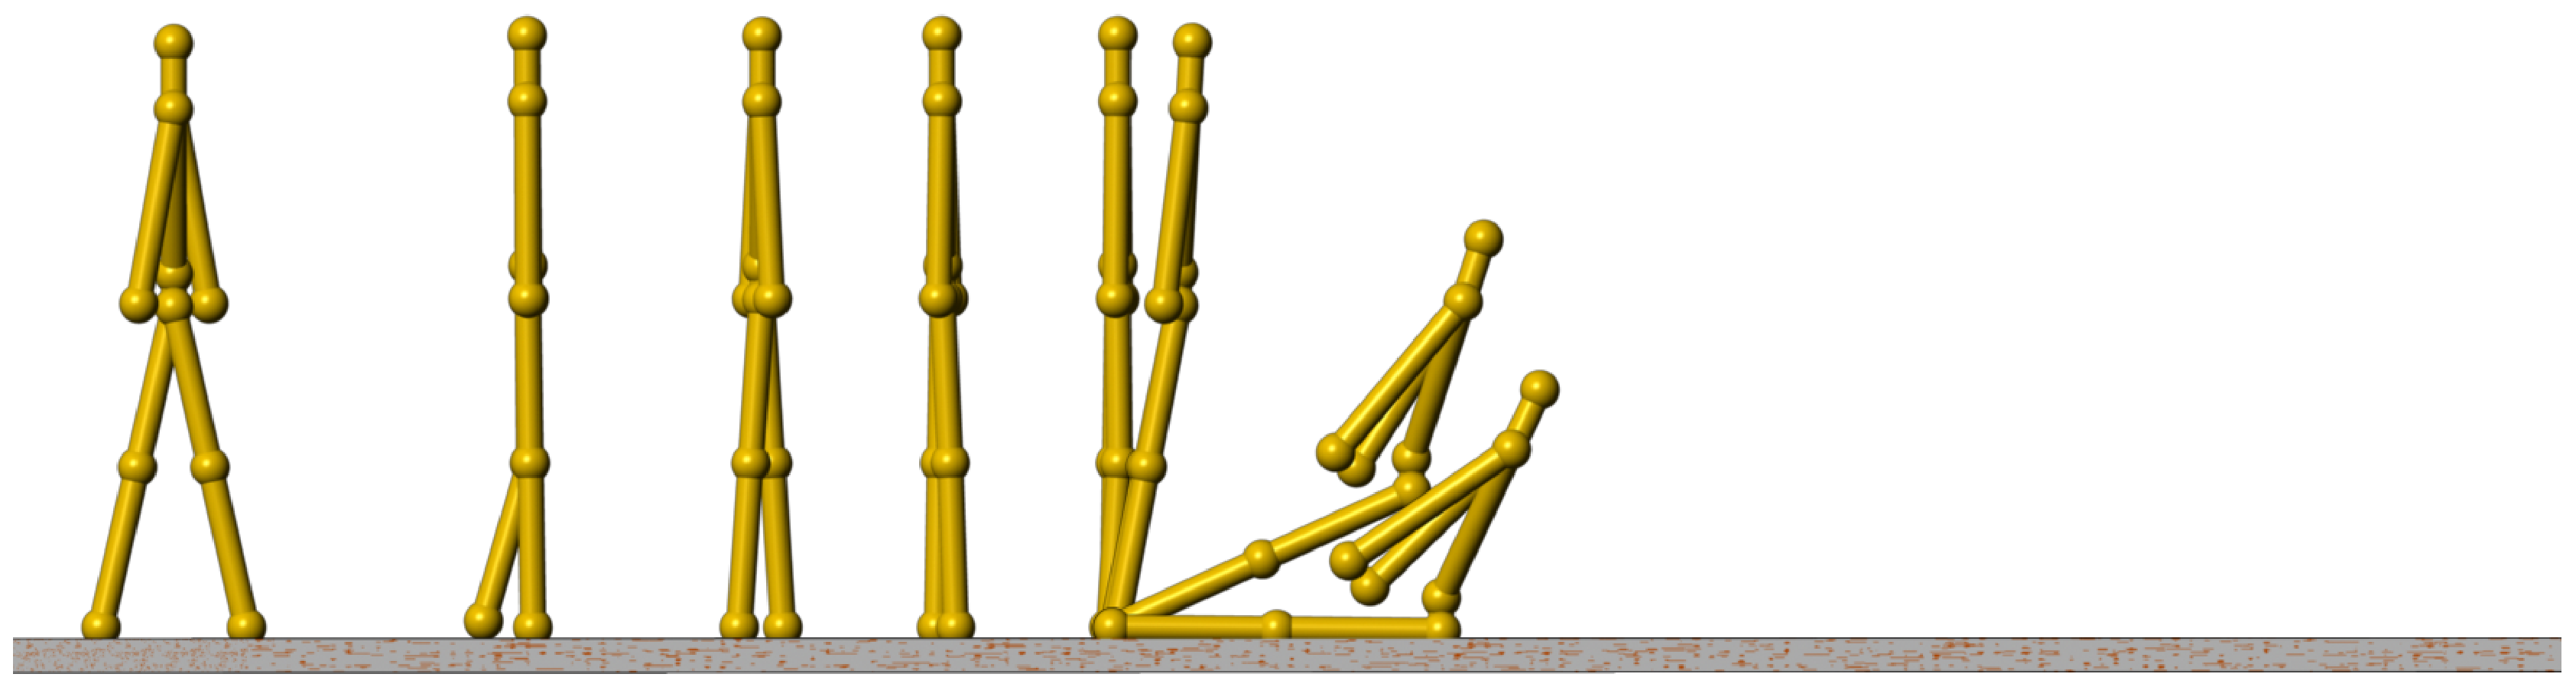
\includegraphics[height=6in]{PlaceHolder}
    \else
      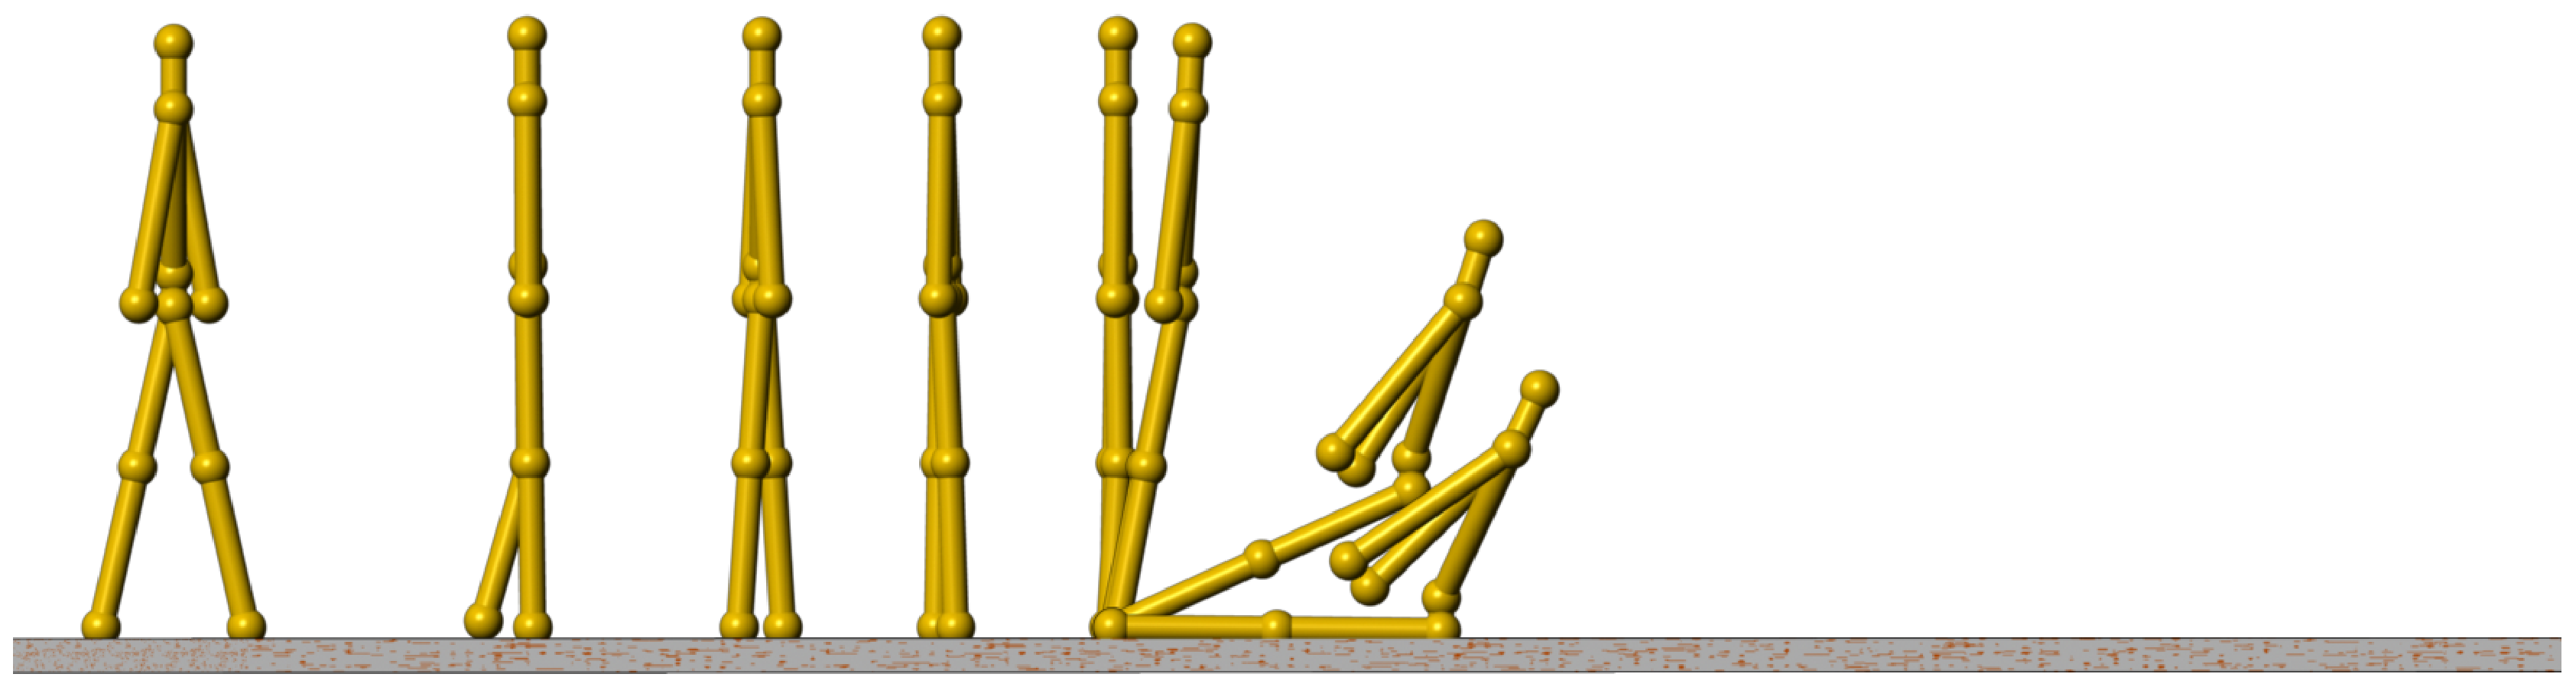
\includegraphics[width=0.7\textwidth]{PlaceHolder}
    \fi
    \caption{Place Holder}
    \label{fig:walkstancebend}
\end{center}
\end{figure}

\subsection{Stance to Walk}
From stance to walk, we must start be making the current state close to the limit circle of walking.
we should place the state of the near the position of start swing position (show in blue).
On the limit cycle of stance, this is the position that the leg is moving forward at maxim speed and the position of the hip is in the middle between the two legs.
if we switch to the walker at this time, then it will begin to walk.



from walking to stance, there the height has to be increase, so there are only one scheme for straight the knees.
the scheme we use is to keep the supporting leg straight then the make the swing leg from bend to straight.

as show in figure
\begin{figure}[!htbp]
  \begin{center}
    \leavevmode
    \ifpdf
      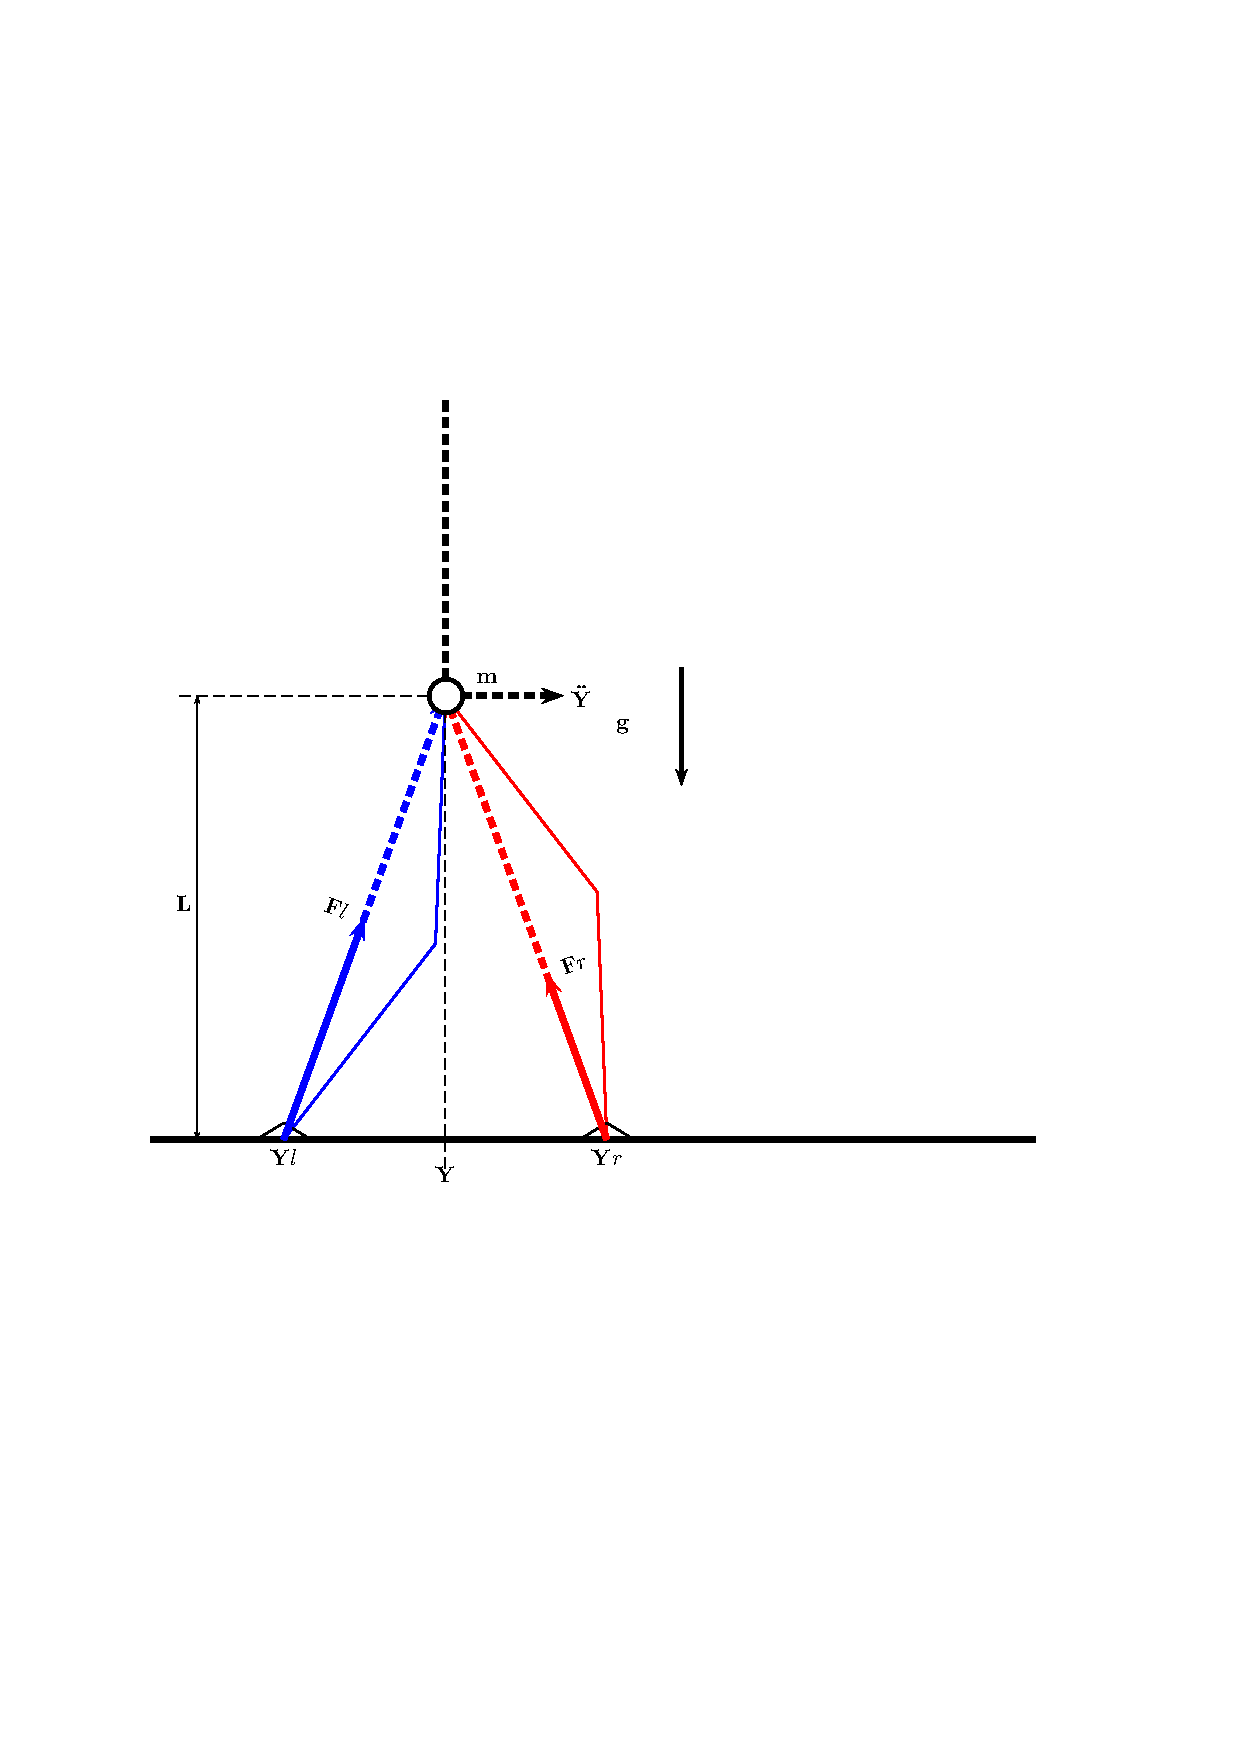
\includegraphics[height=6in]{stancefigure}
    \else
      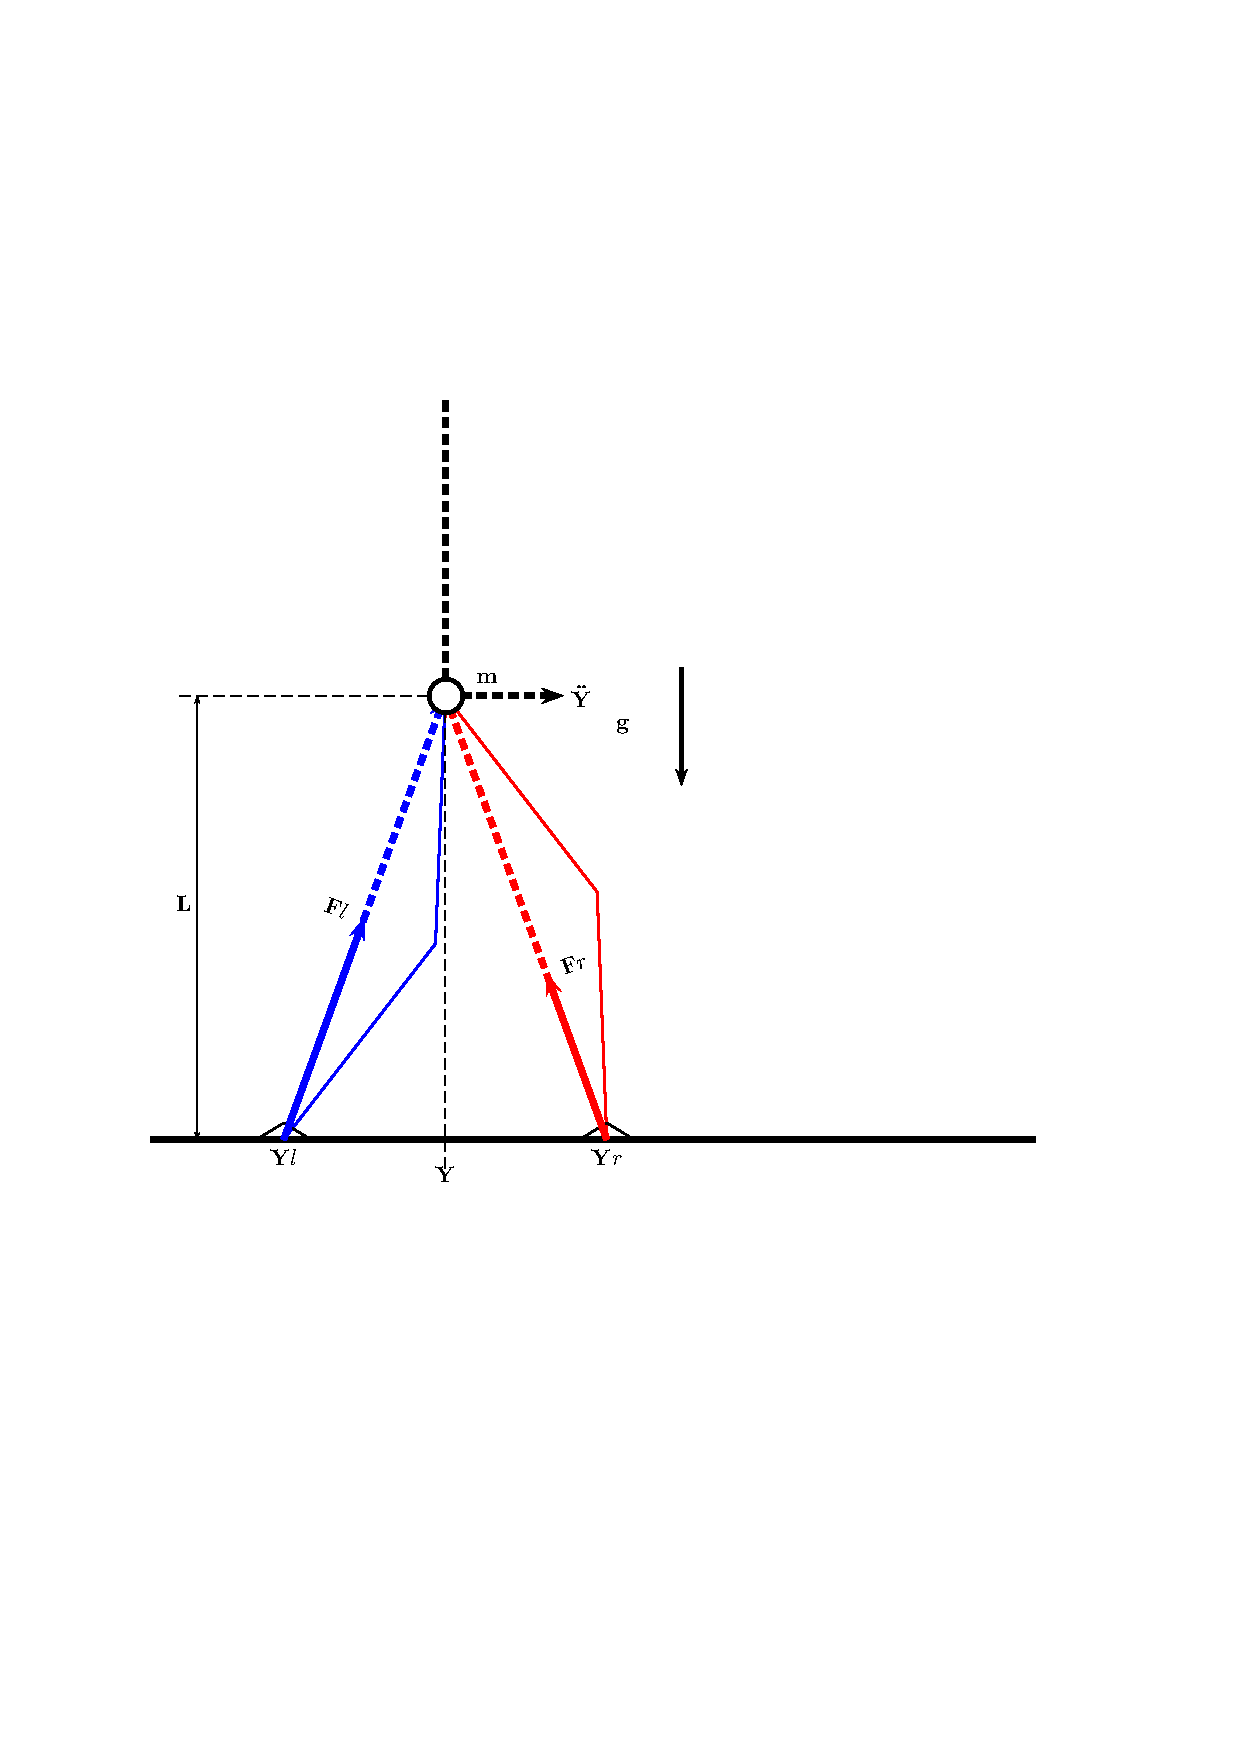
\includegraphics[width=0.7\textwidth]{stancefigure}
    \fi
    \caption{The Place Holder}
    \label{fig:stance2walk}
\end{center}
\end{figure}


A nontrivial problem is when switch from stance to walk, 
we can't make two legs both on the limit circle.
Our approach is put the support leg on the limit circle, for the support leg is more important for maintaining stability.


in the figure above, the stance leg is bit offset of the limit circle, if we put the original swing leg on the limit cycle,for it is going to be the support leg in the following walk step.


\subsection{Speed Action Connection}
When transit from walk to stance, the basin of attraction must include the heel strike state.
original basin of attraction will not include the heel strike; a speed action is needed to enlarge the basin of attraction,
There is an alternative to this, we can lower the walker speed, in this way, and we lower the effort of balance control.

Also, if transition from stance to walk, if little effort is executed, the it will start at pos far from the limit cycle.
then to maintain the stability walking, speed action needed to include for start walking slowing.

So the speed action of stanching and walking must meet some relationship as
\[
\frac{S_s}{S_w}=c
\]

The phenomenon is common for our daily experience; here we give it a mathematical meaning.























